\chapter{Trabalhos Relacionados}

Este capítulo tem como propósito destacar os estudos mais relevantes à proposta de tese e que fizeram parte do caminho percorrido para chegar na proposta final da tese.  A seção 3.1 descreve a minha atuação como professor colaborador, através do estágio docente, para alunos da graduação na disciplina, Fundamentos da Engenharia de Software da UFRJ, em 2018.  A Seção 3.2 detalha a aplicação do Protocolo Copus, desenvolvida durante o acompanhamento de aulas de matemática junto ao Instituto Superior Técnico(IST) com intuito de avaliar a motivação de estudantes. A seção 3.3 detalha a aplicação de um Escape Room também no âmbito do IST junto a estudantes do ensino superior que frequentavam as aulas de lógica de programação e matemática, também para avaliar a motivação de estudantes. Na seção 3.4, é apresentado o resultado das pesquisas relativas a quizzes aplicados em autorregulação da aprendizagem. Na seção 3.5 é apresentado o trabalho realizado junto a análise de dados de cursos da plataforma de MOOC do IST. Na seção 3.6 é detalhado o projeto criado a partir da tese e em parceria entre a UFRJ e o IST, denominado igualdade STEM. Por último, na Seção 3.7 são feitas as considerações finais do capítulo.

\section{Aulas de Fundamentos de Engenharia de Software na UFRJ}

Durante o curso, da disciplina Fundamentos da Engenharia de Software, ministrado no primeiro período de 2018, na Universidade Federal do Rio de Janeiro foram aplicados conceitos teóricos e práticos sobre a engenharia de software, bem como atividades relacionadas ao desenvolvimento colaborativo de software, entre os alunos da UFRJ \citep{github_fes-ufrj_2018}, a comunidade de software público i-Educar \citep{portal_i-educar_2009} e a prefeitura municipal de Caxias, através da secretaria municipal de educação.

Minha atuação foi como professor colaborador, através do estágio docente. Na maioria das vezes em que a disciplina é ofertada os alunos aprendem a parte da teoria, mas sem a experiência de desenvolver um software para um caso real.

Neste sentido, para cumprir os requisitos da disciplina, Fundamentos da Engenharia de Software, os alunos precisaram entregar um projeto completo de \textit{software}, passando pela especificação, desenvolvimento, validação, evolução e testes.  

O projeto teve como base um componente para a comunidade do Software Público i-Educar \citep{portal_i-educar_2009}, como entrega final da disciplina, tendo todo o processo sido documentado através de páginas wiki e o repositório da disciplina no Github \citep{github_fes-ufrj_2018}.

No primeiro mês de aula, foram analisados alguns conceitos básicos sobre Canvas, Métodos Ágeis, \textit{Scrum}, UML, a linguagem Java e seu ambiente de desenvolvimento, a Ide Netbeans e suas funcionalidades, testes e demais conceitos necessários para desenvolver o sistemas dentro deste contexto de aprendizado.

Durante todo o período letivo de aulas, os alunos tiveram a abordagem de sala de aula invertida. Durante as aulas presenciais os alunos tiveram slides de teoria sobre engenharia de software, mescladas com apresentações ao vivo, de forma remota com outros especialistas sobre assuntos diversos usando a ferramenta \textit{appear.in}. 

Além disso, outras aulas presenciais contaram com apresentação de vídeos selecionados da plataforma \textit{youtube}, dinâmicas em grupos, entrevistas com clientes da prefeitura de Caxias, apresentações de outros alunos, preenchimento colaborativo de Canvas e prática do \textit{Scrum}, contendo a)planejamento, b)revisão e c)retrospectiva.

Dentre as atividades, fora da sala de aula, o \textit{HackComb} merece destaque. Durante uma greve na universidade, os alunos perderam uma aula, que foi reposta num dia de feriado, dentro de uma empresa desenvolvedora de software, denominada, Helabs. 

\textit{HackComb} - Hackeando o combustível foi o nome dado a este dia. O nome deste evento é uma adaptação em um formato bem menor de dois conceitos: \textit{Hackathon}. É também uma brincadeira com relação a falta de combustíveis em nosso país. O fato de não existir combustível nos postos, gerou uma greve da faculdade e nos possibilitou usar combustível novo em nosso projeto da disciplina. O que era uma âncora, virou vento favorável e foi o momento de aplicarmos de forma intensa nossa energia usando o tempo a nosso favor.

Durante este dia os alunos tiveram a aplicação da técnica pomodoro  e a participação remota de outros alunos que não puderem estar presentes. Todo o processo de trabalho foi documentado através de página \textit{wiki} da turma, contendo fotos e descrição das tarefas, que se encontram no repositório da turma.  

Abaixo segue a linha do tempo, bem como os conteúdos aprendidos, durante o curso:

\begin{figure}
    \centering
    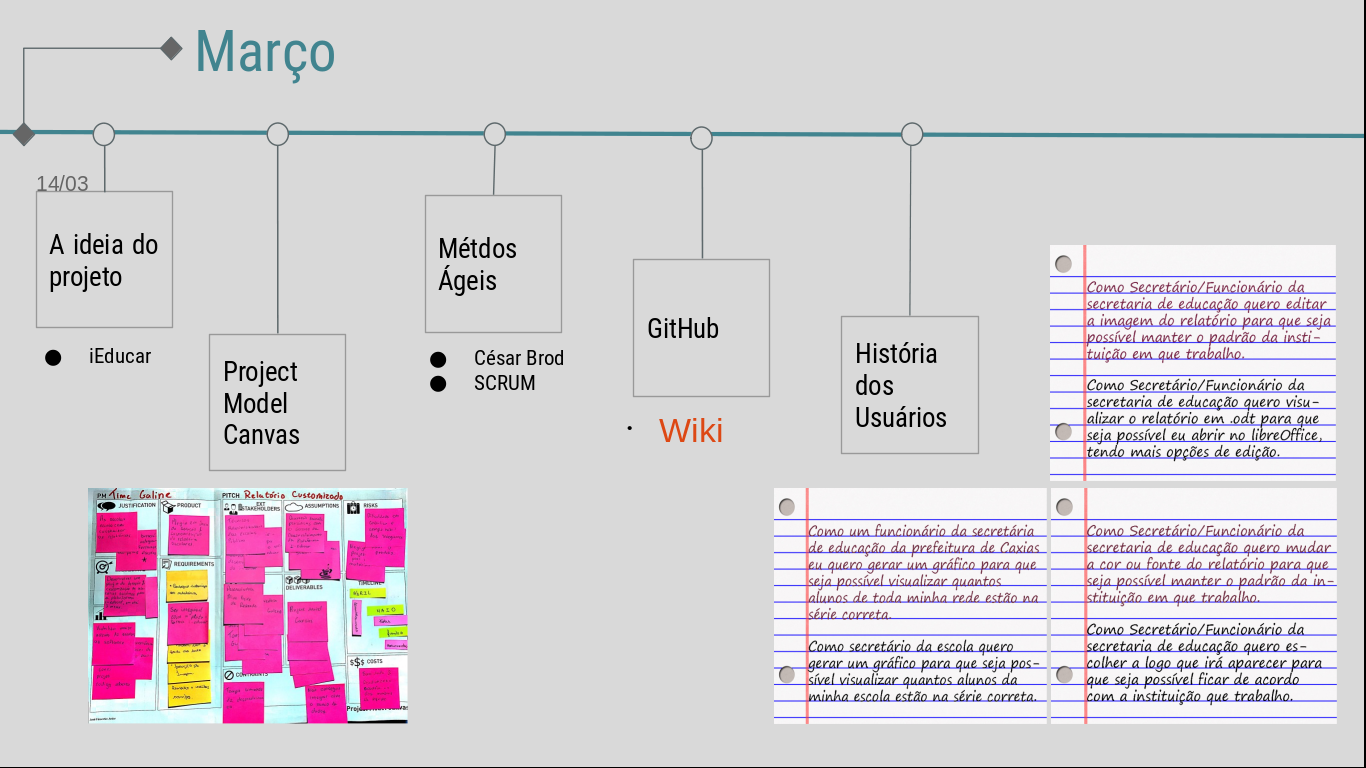
\includegraphics[width=.9\textwidth]{chaps/Images/Linha-tempo1.png}
    \caption{FES-UFRJ - Março-2018.}
    \label{fig:linha-dotempo1}
\end{figure}

\begin{figure}
    \centering
    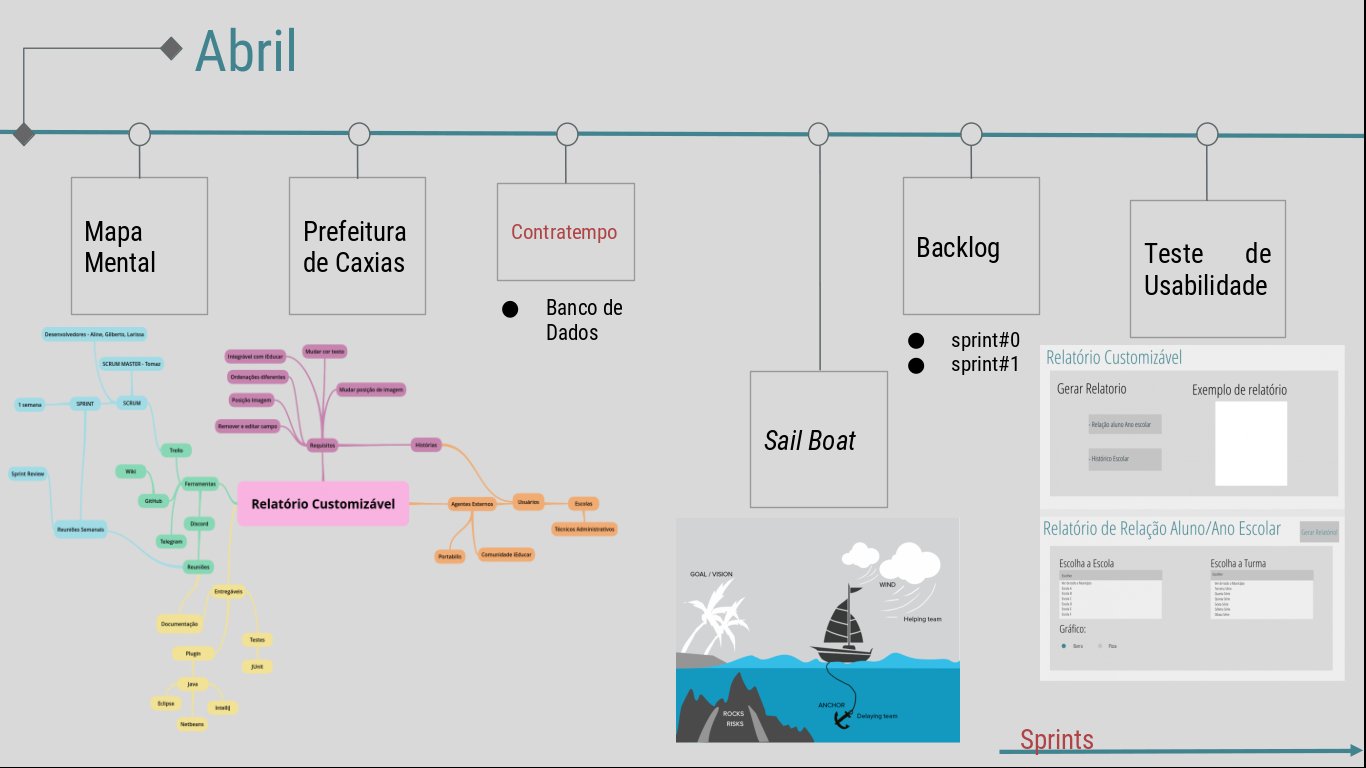
\includegraphics[width=.9\textwidth]{chaps/Images/linha-tempo2.png}
    \caption{FES-UFRJ - Abril-2018.}
    \label{fig:linha-dotempo2}
\end{figure}

\begin{figure}
    \centering
    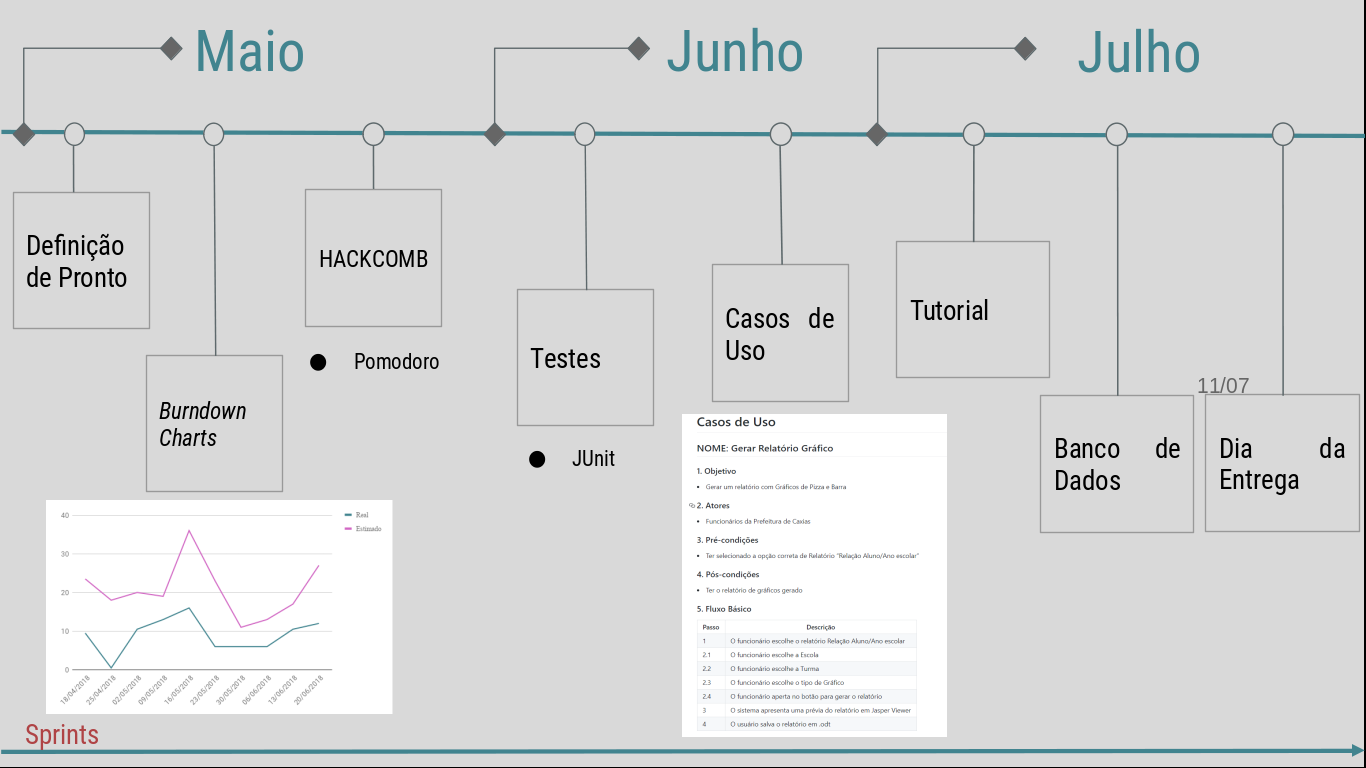
\includegraphics[width=.9\textwidth]{chaps/Images/maio.png}
    \caption{FES-UFRJ - Maio/junho/julho-2018.}
    \label{fig:linha-dotempo3}
\end{figure}


Podemos concluir que os alunos tiveram evolução nas suas habilidades com relação aos temas propostos na aula, conforme uma tabela elaborada por um dos times:

\begin{figure}
    \centering
    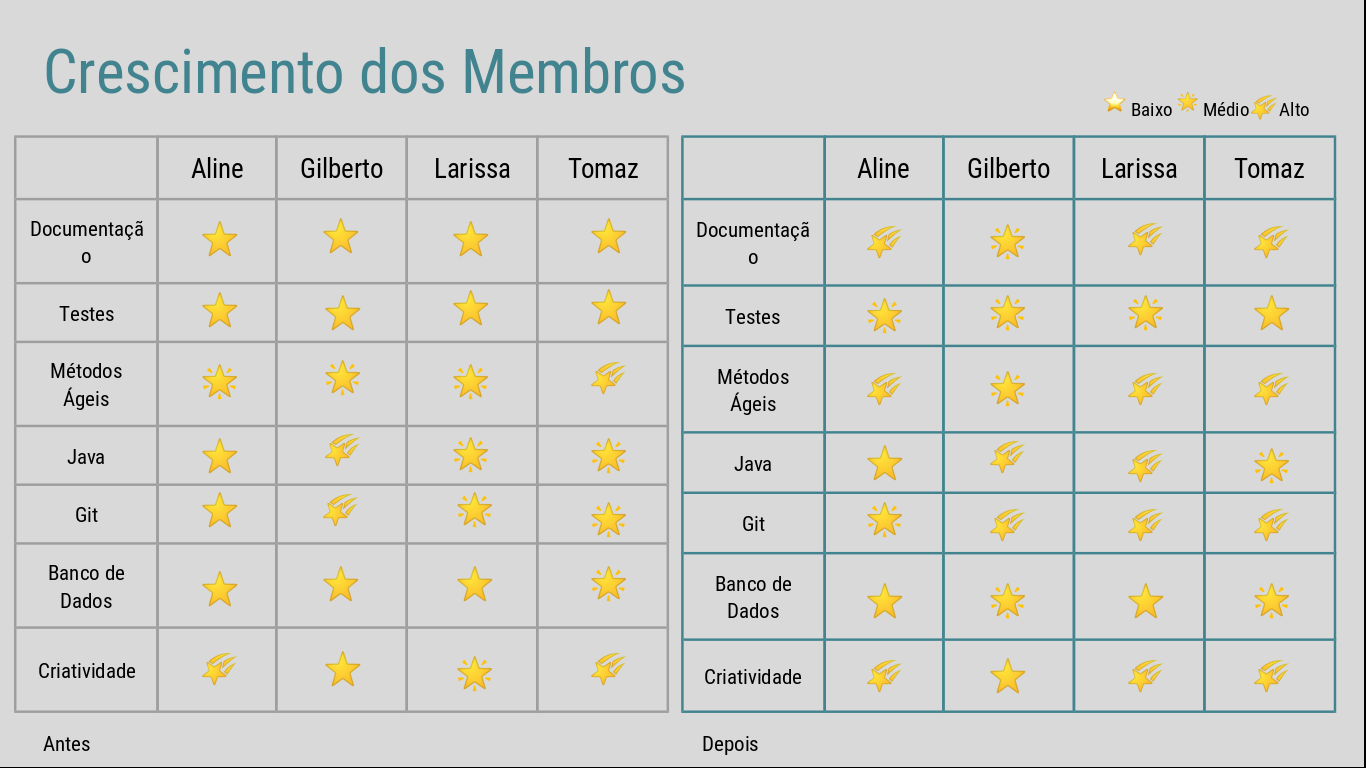
\includegraphics[width=.9\textwidth]{chaps/Images/Habilidades.png}
    \caption{FES-UFRJ - Evolução das habilidades}
    \label{fig:habilidades}
\end{figure}

Todos os times trabalharam com páginas \textit{wiki} de conteúdo aberto que permitiu uma troca de conhecimentos durante as aulas, podendo cada time ver os conteúdos produzidos pelos outros times, também foi disponibilizado um grupo no telegram para continuidade das aulas de forma virtual. Neste grupo existiam a presença de outros especialistas em assuntos diversos, como hackers, desenvolvedores, líderes de comunidades de softwares e especialistas em tecnologia. Todos os alunos compartilhavam suas dúvidas e todos ajudavam. 

Em alguns momentos foram apresentadas tarefas aleatórias com tempo de entrega, onde o primeiro aluno que realizasse a tarefa ganhava uma surpresa, que podia ser um livro, uma camisa ou uma menção honrosa.

Durante as aulas os alunos que conseguiam avançar com alguma atividade, ajudavam os outros que ainda não tinham conseguido realizar. Foram realizadas dinâmicas de meia hora entre os grupos de forma que eles pudessem discutir entre eles algum assunto escolhido para o outro grupo apresentar. Um exemplo disso eram as reuniões virtuais realizadas entre os grupos para ajuda mútua. 

\section{Aplicação do Protocolo Copus}

"Os instrutores e as práticas de ensino que eles empregam desempenham um papel fundamental na melhoria da aprendizagem dos alunos nos cursos de ciências, tecnologia, engenharia e matemática (STEM) da faculdade"(Paper Copus). Em decorrência destas constantes transformações na área da educação, é necessário coletar e analisar informações sobre o que acontece durante o tempo que decorre uma aula. Para que esta análise, principalmente sobre a motivação de estudantes, seja possível, nesta fase da pesquisa usamos um protocolo de observação em sala de aula conhecido como Protocolo de Observação em Sala de Aula para Graduação STEM ou COPUS(Citar). Este protocolo permite que o corpo docente do STEM, após um curto período de treinamento de 1,5 horas, caracterize de forma confiável como o corpo docente e os alunos estão gastando seu tempo na sala de aula(Citar). As aulas monitoradas e preenchidas com a planilha do protocolo(Citar planilha) foram as aulas regulares de Álgebra Linear, ministradas pela Professora Ana Moura Santos na graduação de informática do IST.

Os dados capturados nas observações são referentes a 15 aulas de uma mesma professora e duas outras aulas de dois professores diferentes. As análises que mostraremos abaixo se dividem em três considerando as particularidades da amostra. A primeira análise considera todas as aulas, a segunda somente as aulas da professora com maior frequência, que será nomeada aqui como Professora 1 e a terceira fixa-se somente nos dados das duas aulas dos outros dois professores.

Os dados completos foram analisados à luz de dois algoritmos de classificação baseados em árvore de decisão.
O primeiro algoritmo que foi rodado é o rpart. Por esse algoritmo chegou-se à seguinte árvore simples de decisão mostrada no Gráfico 1.


\begin{figure}
    \centering
    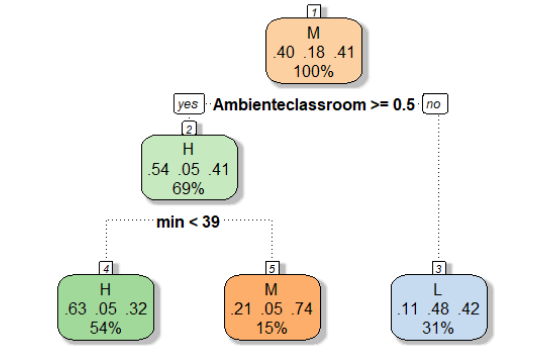
\includegraphics[width=.9\textwidth]{chaps/Images/figura1copus.png}
    \caption{Árvore simples de decisão}
    \label{fig:arvore_simples_decisao}
\end{figure}

A leitura do Gráfico 1 indica que do total das combinações de anotações 41\% são de médio engajamento, 40\% são de alto engajamento e aproximadamente 18\% de baixo engajamento.
Desse total, 31\% dos engajamentos é explicado pelo ambiente de aula ser diferente de sala de aula, ou seja, as aulas acontecem em anfiteatro. Nesses casos, temos que 31\% das combinações referem-se a baixo engajamento.
Para os 69\% restantes há um ponto de decisão referente ao tempo de aula. Até os 39 minutos de aula há uma associação de 54\% das ocorrências para alto engajamento. No caso contrário, há 15\% das associações a médio engajamento.
Temos então que as duas situações mais importantes para o modelo usado, a ponto de aparecerem na árvore de decisão, são o ambiente onde ocorre as aulas e o tempo de aula.
A opção inicial pelo uso da árvore simples deve-se principalmente pelo fato dos seus respectivos modelos serem fáceis de ser interpretados como na figura acima. Para os objetivos desse trabalho que se referem a descrever quais variáveis e quais condições mais influenciam no engajamento dos estudantes, o uso dessa abordagem para uma primeira descoberta é válido. Porém existem outras implementações de uso de árvores de decisão que são mais robustas, principalmente para fazer predições de classificação a partir de dados observados. A desvantagem dessas outras implementações relaciona-se ao fato de não gerarem modelos tão intuitivos. Para este trabalho optou-se por uso de Floresta Aleatória, uma implementação mais robusta de árvores de decisão, para identificar outras variáveis importantes que não tinham sido destacadas quando do uso de árvore simples.
Muito embora o uso de Floresta Aleatória não permita identificar os pontos de gatilho para as decisões, como ocorrem nas árvores simples, foi possível identificar duas novas condições importantes para o modelo. Veja a tabela abaixo.



Pela tabela acima, percebe-se novamente a condição de aula em sala de aula e o tempo de aula, porém agora aparece com destaque mais duas outras condições, uma relacionada a ações dos professores e outra a ação de estudantes, respectivamente FuP e OG.
A importância das quatro variáveis ou condições mais importantes levantadas pelas análises de árvores de decisão podem ficar mais claras através das análises gráficas. As figuras abaixo trazem essa evidência.
O Gráfico 2 mostra a importância do ambiente onde ocorre a aula, especificamente da condição de aula em sala de aula. É possível também perceber a importância do tempo de aula, já que é um gráfico de linha com o tempo representado no eixo horizontal


\begin{figure}
    \centering
    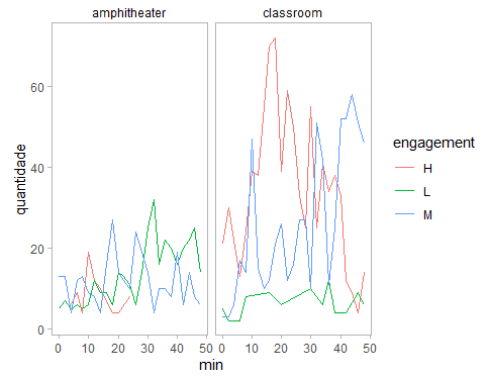
\includegraphics[width=.9\textwidth]{chaps/Images/figura2_copus.png}
    \caption{Árvore simples de decisão}
    \label{fig:arvore_simples_decisao2}
\end{figure}

\section{Aplicação de Escape Room}

Escape Games educacionais são considerados uma estratégia de aprendizado ativo, à medida que os alunos resolvem problemas relacionados com o conteúdo curricular para "escapar" do lugar físico onde eles estão “bloqueados”. Nesta seção é descrita a implementação de dois Escape Games voltados para estudantes de graduação em Ciência da Computação, no Instituto Superior Técnico da Universidade de Lisboa. O procedimento seguido para criar os jogos é apresentado e ambas as atividades são descritas e avaliadas. Além disso, dicas para professores dispostos a construir jogos de fuga educacionais semelhantes são sugerido. Nosso objetivo era entender: a) se os alunos são motivado para este tipo de experiência de aprendizagem; b) se os alunos são ciente dos possíveis ganhos de aprendizagem ao participar nestes Atividades; c) se os alunos, efetivamente, sentem que têm aprendido algo; d) quais são as conquistas desse tipo das atividades (percebidas pelos professores). Considerando o feedback dado pelos alunos: eles se envolvem neste tipo de atividade, estão cientes dos ganhos de aprendizagem e sentem que foi um experiência de aprendizagem frutífera. Além disso, esta atividade foi considerada um sucesso pela corpo docente / equipe organizadora, sendo premiada como uma das boas práticas da universidade.

Embora o ensino tradicional, com base nas aulas tradicionais, tenha sido mostrado ser menos eficaz do que outras alternativas \citep{freeman_active_2014}, no Século 21 continua sendo a principal metodologia de ensino no ensino superior (ES)\citep{wanner_enhancing_2015, yeung_online_2016}. As razões são diversas, nomeadamente que as aulas têm vantagens \citep{webster_defence_nodate}, como transmitir conhecimento em um curto espaço de tempo para um grande número de alunos \citep{gregory_lecture_2013}, garantindo que a transmissão seja correta e precisa. Além disso, muitas vezes falta ao corpo docente a formação pedagógica que facilitam a mudança, como formação pedagógica em ES, ao contrário de outros níveis de ensino, não é obrigatório \citep{jensen_higher_2011}. Na maioria dos países europeus “a maioria dos professores começa a ensinar sem nem cinco minutos de treinamento sobre como fazê-lo ” \citep{rugarcia_future_2000}. Além disso, as políticas universitárias que priorizam publicações / pesquisas sobre o ensino, limitam o tempo e energia disponível para mudar as práticas estabelecidas \citep{waldrop_science_2015}. No entanto, as vantagens dos métodos centrados no aluno, como o aprendizado ativo, estão bem documentadas \citep{prince_does_2004}. Os benefícios da implementação de tais estratégias são o envolvimento dos alunos com o material \citep{ghilay_tbal_2015}, melhor desempenho acadêmico \citep{freeman_active_2014}, "níveis mais elevados de confiança em suas habilidades de resolução de problemas de engenharia" \citep{felder_longitudinal_1997} e menos evasão de alunos \citep{pundak_attitudes_2010}. Dado que “as elevadas taxas de reprovação e evasão dos alunos dos cursos de engenharia têm sido motivo de preocupação para muitas instituições de ensino superior portuguesas” \citep{williams_using_2010}, a aprendizagem ativa representa uma abordagem relevante. Complementarmente, existem recomendações, nomeadamente da Comissão Europeia, para fomentar o desenvolvimento de competências transversais no ES de forma a evitar o “descompasso de competências” (Comissão Europeia, 2012) entre o que a indústria exige dos licenciados e o que os alunos aprendem. Essas habilidades transversais incluem trabalho em equipe, comunicação, criatividade, autorregulação e resiliência. Considerando que os alunos de hoje passam um tempo significativo jogando jogos, a introdução de elementos de jogos na educação - aprendizagem baseada em jogos - é uma tendência crescente em ambientes educacionais, incluindo ES \citep{clarke_escaped_2017}. Os Jogos Educacionais de Escape Room reúnem os benefícios educacionais da aprendizagem ativa, o desenvolvimento de habilidades transversais, a colaboração e a alegria de jogar. Aproveitando a dinâmica do jogo e criando um ambiente de aprendizagem envolvente, no qual os alunos se comunicam e trabalham em equipe para resolver diversos problemas relacionados com os conteúdos, foram implementados dois Escape Games com alunos de Informática (CS), no Instituto Superior Técnico da Universidade de Lisboa. Essas atividades aconteceram nos cursos de Lógica para Programação (LP), nosso estudo piloto, e Álgebra Linear (LA). A partir de agora nos referiremos à primeira experiência como EscapulISTe? -LP e a última como EscapulISTe? -LA. Nossas perguntas de pesquisa foram:

\begin{itemize}
    \item RQ1: Os alunos estão motivados para este tipo de aprendizagem experiência?
    \item RQ2: Os alunos estão cientes dos ganhos de aprendizagem desses Atividades?
    \item RQ3: Os alunos sentem que podem aprender com o Escape Game?
    \item RQ4: Quais são as principais realizações de acordo com o professores?
\end{itemize}

Nesta seção, damos uma descrição detalhada do procedimento que seguimos na criação e implementação Escape Games, com o objetivo de compartilhar o que percebemos como bom práticas e "não fazer" a serem evitados durante a preparação de essas atividades. Assim, esperamos que nossos experimentos possam ajudar outros professores de ES a se concentrarem na importância de se divertindo enquanto prepara uma atividade para envolver seus alunos sobre o assunto. Esta seção está organizada da seguinte forma: Começamos com um contexto teórico explicando porque Escape Games constituem uma estratégia de aprendizagem ativa valiosa em educação STEM (Sub-Seção 2). Na Sub-Seção 3, as duas implementações de Escape Games (EGs) são descritas. Na Sub Seção 4, a avaliação de ambos os jogos é apresentada, e na Sub-Seção 5 nós apresentamos as lições aprendidas durante sua criação e implementação. Encerramos apresentando algumas conclusões e trabalhos futuro (Sub-Seção 6).

\subsection{Bases Teóricas}

A aprendizagem ativa pode ser definida como "qualquer curso relacionado que todos estudantes em uma sessão de aula são chamados a fazer além de simplesmente assistir, ouvir e tomar notas ”\citep{felder_active_2009}. Estratégias de aprendizagem ativa promovem a atividade do aluno e a motivação \citep{prince_does_2004}. Sua implementação em uma classe varia de pausando uma palestra para propor um exercício rápido ou mesmo mudando completamente a dinâmica da classe. Um EEG em que os quebra-cabeças são preparado para fazer os alunos aprenderem algo novo ou praticarem aprendizagens anteriores é uma aprendizagem ativa. Além disso, estudantes  colaboram uns com os outros para resolver os quebra-cabeças. A colaboração pode alavancar a aquisição de outros tipos de conhecimento, como a interação social promovendo a aprendizagem de técnicas e habilidades transversais \citep{tadjer_improving_2020}.

EGs são definidos como jogos baseados em equipes de ação ao vivo (geralmente 5 a 7 pessoas), onde os jogadores descobrem pistas e resolvem quebra-cabeças, “Trancado” em um cômodo ou casa, para cumprir uma meta específica (geralmente escapando), em um período de tempo limitado e normalmente de uma hora \citep{nicholson_peeking_2015}. Eles foram apresentados ao público como atividades recreativas, mas logo a emoção se espalhou para áreas educacionais. Quando aplicado à educação, os EEGs promovem o desenvolvimento de habilidades transversais, como trabalho em equipe e comunicação eficaz porque, em vez de jogar atrás de uma tela, participantes estão colaborando com pessoas reais \citep{nicholson_creating_2018} em tempo real e trabalhando para atingir um objetivo comum. Pensar de forma criativa é crucial neste processo, pois eles encontram diferentes desafios que precisam ser resolvidos de novas maneiras \citep{wiemker_escape_2015}. Resiliência e a autorregulação também são incentivadas, pois diversos estudos relatam que os alunos se sentem frustrados durante a atividade \citep{hermanns_using_2017}.

Embora os autores apresentem isso como uma lacuna, a sensação de frustração é comum, não só ao jogar, mas também em múltiplas situações de vida. Portanto, se devidamente explorado e preparado, participar do EG ajuda o jogador a implementar a auto-regulação, para manter uma postura calma diante dos outros, e continuar trabalhando na solução apesar da frustração. A capacidade de entregar resultados sob pressão é uma habilidade com alta demanda no mundo da engenharia \citep{harun_employability_2017}. Além de ajudar a consolidar conhecimentos e valorizar habilidades transversais, EEG são essencialmente jogos. Alunos nascidos em um mundo de tecnologia massificada, tem acesso a um abundância de plataformas de entretenimento digital que antes gerações não possuiam \citep{osmanovic_beyond_2016} e são parte de uma rede hiperconectada da sociedade digital \citep{buitrago-ropero_digital_2020}. Os EEGs representam uma fonte de motivação devido à semelhança com outros tipos de jogos. Por isso parece correto aplicá-los em um ambiente universitário, dado seu “apelo e valor educacional” \citep{clarke_escaped_2017}.

Houve várias implementações de EEG em ES com resultados promissores. Em um estudo desenvolvido com estudantes de farmacologia \citep{hermanns_using_2017}, 72,2\% dos participantes reconheceram que aprenderam os conceitos abordados durante o jogo e afirmou que a atividade lhes permitiu pensar fora do caixa. Em uma experiência baseada em nutrição saudável \citep{yachin_promoting_2019}, os autores encontraram um aumento após a participação com significância estatística, não apenas no número de respostas corretas a um pós-questionário (em todas as perguntas, exceto uma), mas também na automotivação dos alunos. Dos alunos participando de um eletroímã EG \citep{hou_exploring_2012}, 74\% relataram ter entendido melhor o assunto com o jogo do que com livros didáticos; e em um ambiente de robótica educacional, a maioria dos participantes reconheceram a “usabilidade como ferramenta de ensino” do EG \citep{giang_exploring_2020}. Em um ambiente de química \citep{dietrich_escape_2018}, a maioria dos participantes indicaram que a atividade ajudou a desenvolver a construção da equipe (96\%) e comunicação (90\%).

\subsection{Implementando Escape Games Educacionais}

A preparação complexa envolvida neste tipo de jogos é muitas vezes considerado uma desvantagem potencial \citep{wiemker_escape_2015}, como a maioria dos professores não são especialistas em EG. No projeto atual, duas funções principais dentro a equipe organizadora foi criada - o designer e o professor com experiência no conteúdo (a partir de agora, conteúdo especialista). Essa escolha ajudou a lidar com a complexidade, pois o especialista em conteúdo não está envolvido no design do jogo e o designer não precisa pensar sobre o desafio específico. No entanto, os desafios e seu fluxo, muitas vezes precisam ser repensado pelo designer, de acordo com as instruções do conteúdo de especialistas, pois o especialista é aquele com o conhecimento para decidir o que vai levar à melhor experiência pedagógica. Assim, alguma negociação é necessária entre as partes. A criação e implementação de ambos os EEGs é apresentada no próxima seção.

\begin{figure}
    \centering
    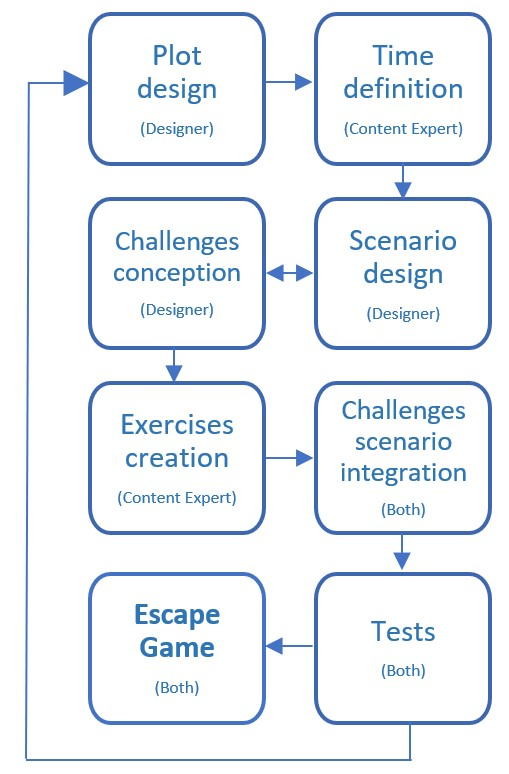
\includegraphics[width=.9\textwidth]{chaps/Images/Esquema Escape(1).jpg}
    \caption{Construindo o Escape Game Educacional.}
    \label{fig:esquema_escape}
\end{figure}

\subsection{Procedimento Geral}

O procedimento seguido pode ser visualizado na Figura 1. Em uma primeira etapa, o designer define o enredo do jogo e o especialista em conteúdo decide quando a experiência deve ocorrer. Uma vez que essas restrições sejam estabelecidas, o designer pode funcionar no cenário - depende da história, mas também do orçamento - e conceituar os desafios. O número de desafios deve ser definido juntamente com o resultado de cada desafio dentro do fluxo do jogo \citep{csikszentmihalyi_creativity_1996}. Por exemplo, o designer pode decidir que a saída do desafio 1 abre um armário com três números e o desafio 2 prompts de saída a senha. Em seguida, o especialista em conteúdo é solicitado a criar N exercícios, um para cada desafio. Por exemplo, considerando o exemplo anterior, o especialista em conteúdo cria exercícios de forma que o o primeiro resultado do exercício corresponde a três números, e o o segundo exercício retorna seis letras e três números (ou seja, um senha).

Em seguida, os desafios são implementados no cenário real, e o jogo está pronto para ser beta testado, preferencialmente por alunos com a mesma formação dos participantes finais. Um desafio frequentemente citado na literatura é que alguns jogadores aprendem as regras do jogo ao invés dos conteúdos educacionais \citep{sanchez_teaching_2019}, criando uma experiência superficial \citep{nicholson_creating_2018}. Este aspecto pode ser minimizado com uma definição prévia de resultados de aprendizagem rigorosos e objetivos \citep{waldrop_science_2015}, mas também com um debriefing cuidadoso no final da atividade para garantir a reflexão e metacognição \citep{sanchez_teaching_2019}. Isso pode ser feito durante os testes beta, o que pode levar a alterações em todo o conjunto de etapas anteriores. Obter feedback de testadores e participantes e refletir sobre a experiência pode ajudar o designer e o especialista em conteúdo realizarem rearranjos e correções. Além disso, após as implementações iniciais, os professores podem construir mais confiança para ampliar a experiência \citep{borrego_room_2017}. Ainda nesta etapa de validação, e antes de apresentar o jogo final aos alunos, uma última ação deve ser realizada: uma diretriz detalhada deve ser fornecida e testada pela equipe organizadora, ou um membro da equipe, que será responsável por preparar a sala após cada implementação.

Todo o rearranjo de ações necessário deve ser detalhado com precisão em uma lista ordenada, que deve ser rigorosamente seguida. Só então o EEG está pronto para ser executado (passo 6). Porém, ainda existem alguns procedimentos a serem seguidos. Em cada sessão, um dos organizadores da equipe se reúne com a equipe de cada aluno e explica o enredo. Nesse momento, os alunos são convidados a assinar um formulário declarando que não vão discutir a atividade com outros alunos e que cuidarão bem dos materiais. Após cada implementação do jogo, ou o professor se reúne com a equipe dos alunos para um breve debriefing, ou uma pesquisa pode ser aplicada a fim de garantir que os alunos refletem sobre a atividade e reconhecem possíveis aquisições de outras habilidades. Depois que todas as equipes participarem, é proposto um questionário a todos os alunos, a fim de avaliar a atividade.

\subsection{Plot Design e Definição do tempo}

Uma narrativa que ajuda a “Definir a atmosfera do jogo e estabelecer as bases do investimento emocional e da curiosidade junto com o jogador" \citep{clarke_escaped_2017} é uma peça importante no projeto de EEG. No nosso caso, um personagem foi criado: Anita, uma estudante de Ciência da Computação que adora EG. Em EscapulISTe? -LP, estudantes se reuniram no quarto de Anita para estudar Lógica. Eventualmente, eles adormecem. Então acordam para descobrir que Anita os trancou e deixou vários desafios de LP que eles precisam resolver para escapar da sala. Eles têm uma hora para fazer isso, ou será tarde demais para o exame. O EscapulISTe? -LP foi implementado no final do semestre e antes do primeiro exame. Portanto, os alunos podem relembrar os principais tópicos antes de se preparar para o exame e testar seus conhecimentos prévios.

Em relação ao EscapulISTe? -LA, Anita fica trancada dentro do armário enquanto prepara um EEG sobre LA. Ela manda um e-mail pedindo ajuda. Os estudantes devem resolver os desafios para abrir o armário e ter uma hora para fazê-lo, ou ela não conseguirá respirar e morrer. EscapulISTe? -LA foi planejado para ser implementado antes do teste intermediário. Essa escolha se baseou em dois motivos. Em primeiro lugar, os desafios estavam relacionados aos conceitos algébricos que possuem saídas numéricas. O segundo motivo para esse planejamento foi pedagógico - no momento do teste de meio de semestre, os alunos geralmente estão sobrecarregados com os projetos de outros cursos e têm um desempenho pior, em comparação com o primeiro teste.

\subsection{Scenario design}

Todos os elementos do EEG devem ser integrados em um conjunto coerente que promova uma experiência envolvente e significativa. O espaço físico e a narrativa devem ser combinados, com a ajuda de decorações e objetos \citep{guigon_model_2018}, para criar um enredo plausível. Nosso primeiro desafio foi criar uma sala de Anita confiável. Isso foi possível com a doação de diversos móveis. Além disso, definimos traços em relação à “personalidade” de Anita: ela adora a seleção nacional de futebol, livros e Harry Potter. Detalhes da decoração como uma foto da seleção nacional e uma camiseta de Harry Potter foram introduzidos. O cenário para LP pode ser visto na Figura 2.

\begin{figure}
    \centering
    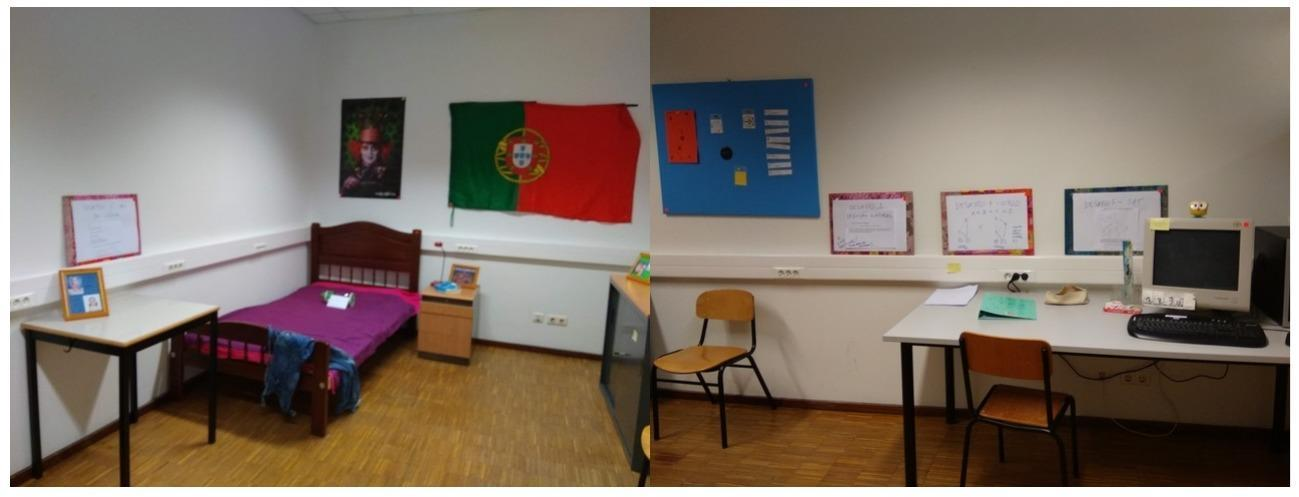
\includegraphics[width=.9\textwidth]{chaps/Images/Figura2(1).jpeg}
    \caption{Quarto da Anita}
    \label{fig:quarto_anita}
\end{figure}

\subsection{Challenges conception}

Ao contrário do que se pode constatar no EG ao vivo e dados os objetivos pedagógicos, é contraproducente o aluno perder tempo com pistas falsas. Assim, em ambas as implementações, os alunos tiveram cinco exercícios para resolver, explicitamente numerados. Posteriormente, foi definido o fluxo dos cinco desafios, determinando, por exemplo, que o primeiro abrisse o armário X que permitiria aos alunos o acesso ao segundo desafio, com uma ordem estrita de ações. As fechaduras estavam presas a um carrinho, uma mochila, uma maleta e duas caixas. Alguns deram chaves para abrir a gaveta da mesinha de cabeceira ou do guarda-roupa, onde os alunos encontravam os exercícios escritos.

A integração do EEG em áreas não numéricas pode representar um desafio adicional, pois as soluções para abrir as fechaduras são geralmente numéricas \citep{guigon_model_2018}. Em nossa experiência, mesmo em cursos STEM, às vezes o tipo de exercícios não se ajusta precisamente a uma meta numérica. Sempre é possível, em qualquer conteúdo, adotar uma abordagem criativa onde as palavras se transformam em números e explorar outras maneiras de desbloquear fechaduras.

\subsection{Exercises creation}

Após a definição do número de desafios e seu fluxo, os especialistas em conteúdo criaram os exercícios para seu tópico de especialização, considerando as orientações fornecidas pelo designer. A concepção dos exercícios baseou-se nos objetivos de aprendizagem traçados para o EEG. Para álgebra linear (EscapulISTe? -LA), por exemplo, cinco objetivos de aprendizagem foram estabelecidos:

\begin{itemize}
    \item Manipulando equações da matriz
    \item Inversos de matriz de computação
    \item Aplicação de propriedades de matrizes de Markov
    \item Determinantes de computação
    \item Manipulação de matrizes particionadas
\end{itemize}

Em seguida, foram preparados diferentes exercícios de álgebra de matrizes, matrizes inversas, matrizes de bloco e determinantes. Aqui estão dois exemplos de exercícios específicos:

\begin{itemize}
    \item Considere a matriz simétrica [fornecida explicitamente]. Você precisará descobrir as entradas da terceira coluna da matriz inversa.
    \item Considere a matriz de Markov [fornecida explicitamente com três entradas ausentes] com o vetor estacionário .... (OOPS, você precisa descobrir!). A chave que você precisa encontrar é composta pelas entradas ausentes na matriz.
\end{itemize}

Para EscapulISTe? -LP, os exercícios propostos progrediram da dedução natural e representação lógica de primeira ordem para diagramas de decisão binários ordenados. Além disso, um programa em Prolog (com um bug) foi fornecido. Quando o bug foi corrigido, um número foi retornado e os alunos puderam acessar o próximo desafio.

\subsection{Challenges scenario integration}

Inúmeras ideias de desafios podem ser implementadas. Aqui são três exemplos usados no projeto atual:

\begin{itemize}
    \item Um dos números abre uma caixa com um ímã dentro. Este ímã permite que os alunos removam uma chave no fundo de uma caixa transparente longa e estreita.
    \item Aproveitando o fato de que a lógica estava sendo ensinada, os alunos precisaram decifrar três fórmulas na lógica de primeira ordem para encontrar a ordem de três xícaras numeradas.
    \item Tinta invisível foi usada para escrever informações importantes sob a cama de Anita. Durante o jogo, os alunos encontraram uma lanterna de luz negra e uma pista do livro de Calvin e Hobbes, "Monstros debaixo da cama".
\end{itemize}

\subsection{Beta tests}

Antes da implementação final com os alunos, professores voluntários testaram ambos os jogos. Muitas pistas foram repensadas na época. Para EscapulISTe? -LP, nosso estudo piloto, cinco alunos de CS também foram convidados a jogar o jogo. Com o feedback deles, conseguimos entender quais desafios eram muito complicados ou muito fáceis. Para o EscapulISTe? -LA, vários alunos de diferentes anos e graus se ofereceram para testá-lo. Um debriefing ocorreu após cada sessão experimental e o feedback geral permitiu uma reflexão sobre a experiência e promoveu várias correções. Em relação às orientações para reorganizar a sala, o designer do jogo forneceu uma lista detalhada com os códigos do armário e as 25 etapas necessárias para ter todos os objetos na posição correta. Esta foi uma peça fundamental e professores / equipe organizadora responsáveis pelas implementações praticaram a tarefa de antemão, várias vezes. Se algo falhasse, a próxima implementação seria comprometida.

\subsection{Avaliação}

\subsection{EscapulISTe? -LP Feedback dos alunos}

EscapulISTe? -LP foi o piloto e o objetivo principal foi obter insights a partir da experiência. Sete equipes (3-6 alunos) participaram (um total de 33 alunos do primeiro ano de CS), até o final do semestre da primavera. Se algum dos desafios for muito complicado, eles adicionam acesso a “spoilers”, já que as soluções dos desafios foram escritas no verso de quadros coloridos (Figura 2). Após cada sessão, um breve debriefing foi feito. Alguns dos grupos marcaram um ou dois “spoilers”, mas a maioria dos alunos conseguiu “escapar” sem ajuda, geralmente em cerca de 45 minutos.

Os alunos foram convidados a dar feedback informal, com a possibilidade de anonimato. Temos 24 respostas, e apenas comentários positivos como: “foi muito bom! [...] reveja o materiais [...] realmente criativos ”,“ Foi uma experiência legal. [...]
muitos tópicos foram revisados [...] formas alternativas de estudar,
mais divertida e também diferente ”,“ Legal !!!! ”.

\subsection{Avaliação do EscapulISTe? -LA}

O EscapulISTe? -LA foi proposto aos 90 alunos matriculados no primeiro ano de Ciência da Computação, em novembro de 2019, antes do exame de meio de semestre. Embora a atividade fosse opcional, teria um impacto irrisório na nota final (cerca de 1,5\%). Aconteceu durante oito dias da semana, duas equipes por dia. Os alunos foram organizados em equipes (5 alunos cada), inscrevendo-se previamente num sistema de matrícula desenvolvido por um aluno bolseiro. Este registro online facilitou a organização das equipes de alunos por vagas disponíveis e nos permitiu manter um registro da participação dos alunos. Dos 90 alunos, 79 alunos se inscreveram para a atividade. Desta vez não houve “spoilers” e cada grupo demorou entre 40 a 55 minutos para resolver os desafios. Novamente, após cada sessão, um breve debriefing foi feito. Quando todas as equipes terminaram a atividade, um questionário foi realizado através do nosso Sistema de Gestão de Aprendizagem (LMS). Dos 90 alunos, foram coletadas 66 respostas (8 mulheres e 58 homens), 63 respostas de alunos que participaram do EscapulISTe? -LA e 3 de alunos que não participaram. Além disso, em conversas informais com os organizadores, eles puderam compartilhar sua experiência sobre se sentirem às vezes frustrados durante a atividade, mas felizes por terem superado isso com a ajuda do grupo.

\subsection{EscapulISTe? -LA Feedback dos alunos}

A seguir, analisamos as respostas às nossas perguntas de pesquisa.
1) RQ1: Os alunos estão motivados para esse tipo de experiência de aprendizagem?
A fim de entender o que motivou os alunos a participar, eles foram solicitados a indicar os motivos pelos quais optaram por fazê-lo (como mencionado anteriormente, esta atividade era opcional). A seguinte questão de checkbox foi fornecida (várias opções podem ser escolhidas simultaneamente, então a soma é acima de 100\%): “Qual foi a sua principal motivação para participar?”

\begin{itemize}
    \item I'm a fan of EG (25.6\%)
    \item I’m counting on it to improve the grade (28.6\%)
    \item It seemed like a fun opportunity to learn (37.6\%)
    \item I just wanted to relax (8.3\%)
Other (0\%)
    
\end{itemize}

Observe que nenhum aluno escolheu “Estou contando com isso para melhorar a nota "como a única opção, o que significa que eles não eram
fazer a atividade “só” para melhorar a nota.

2) RQ2: Os alunos estão cientes dos possíveis ganhos de aprendizagem dessas atividades?
A fim de avaliar RQ2, a seguinte questão foi fornecido (novamente, várias opções podem ser escolhidas):“Como você acha que este tipo de atividade pode ajudá-lo a aprender o assunto?"

\begin{itemize}
    \item Envolvendo meu esforço individual, preciso saber o assunto a contribuir para o sucesso do grupo (30,7\%)
    \item Usando interações em grupo para resolver desafios, eu avanço mais rapidamente na compreensão do assunto (37,0\%)
    \item Sendo uma atividade divertida e descontraída, sou mais motivado para aprender (32,3\%)
    \item Não acho que aprendemos nada com esse tipo de atividade (0\%)
\end{itemize}

Embora aponte para diferentes motivos (motivados individualmente ou devido ao trabalho da equipe), todos os alunos podem achar este tipo de atividade valiosa do ponto de vista das conquistas de aprendizagem e desenvolvimento de habilidades. É interessante verificar que alguns alunos consideraram que fazer parte de uma equipe era uma motivação para aprender, seja na perspectiva de ajudar a equipe (30,7 \%), seja individualmente (37,0 \%).

3) RQ3: Os alunos acham que podem aprender com Escape Game? 

Para avaliar o RQ3, foi feita a seguinte pergunta de caixa de seleção: “Se você participou, em que medida você acha que o escapulISTe ajudou você?”

\begin{itemize}
    \item Envolvendo meu esforço individual, preciso saber o assunto a contribuir para o sucesso do grupo (30,7\%)
    \item Ganhei confiança no meu conhecimento do assunto (43,4\%)
    \item Foi apenas uma atividade divertida (15,5\%)
    \item Não acho que tive nenhum ganho significativo (3\%) 
\end{itemize}

As respostas a essa questão reforçam que o EEG, como estratégia ativa de aprendizagem, pode ajudar os alunos a ganhar confiança em seus conhecimentos (43,4\%) e é importante para aumentar a consciência das falhas de compreensão (38,2\%). Além disso, dos dois alunos (3\%) que responderam que não encontraram nenhum ganho importante com a atividade, um deles considerou que se tratava de “uma atividade lúdica” (contribuindo com 15,5\%).

4) RQ4: Quais as principais conquistas de acordo com a equipe organizadora?
Embora as notas nos testes intermediários também tenham sido particularmente altas em comparação com anos anteriores de implementações de LA, não podemos concluir que os bons resultados dos alunos foram uma consequência direta da atividade de EEG, uma vez que esta atividade foi combinada com uma nova avaliação formativa baseada em 10 quizzes online com feedback automático \citep{santos_assessment_2017}, e uma estratégia de sala de aula invertida melhorada com base em um MOOC \citep{nicholson_peeking_2015}.

No entanto, juntamente com um desempenho de alto nível nos testes escritos, o feedback dos alunos apóia a ideia de que o EEG pode ser usado para atingir os objetivos de aprendizagem dos alunos, se divertindo e desenvolvendo habilidades transversais como o trabalho em equipe e a autorregulação. Além disso, ao responder a um questionário final sobre o curso de LA, na questão “A atividade foi um momento importante na sua aprendizagem?”, 84,9\% dos alunos indicaram que foi, sim, importante para a sua aprendizagem. Além disso, também comentam que “Esse tipo de atividade deve ser repetido com mais frequência, pois incentiva o estudo do assunto, promove a cooperação e tudo de uma forma divertida". Diversas respostas de uma questão aberta do questionário corroboram a visão positiva deste aluno: “Achei interessante a atividade da sala de fuga, por utilizar o material de forma lúdica e interativa. [...] deveria haver mais atividades desse tipo "; “Adorei muito a ideia do Escape Game”; “Acho que ideias fora da caixa, como o Escape Game, são amplamente aceitas pela comunidade estudantil e também o caminho para um aprendizado mais atraente”. Concluímos que o principal desafio desta atividade é escalabilidade. O curso de LA, por exemplo, é um curso obrigatório oferecido pelo Departamento de Matemática a cerca de 1.500 alunos de diferentes cursos de Engenharia. Seria extremamente exigente divulgar esta atividade a todos os alunos.

\subsection{Lições Aprendidas}

Existem vários guias disponíveis \citep{ho_unlocking_2018, wiemker_escape_2015} que podem ajudar na fase de preparação e configuração de um EEG. Durante a implementação de ambos EscapulISTe?, realizamos várias ações que nos fizeram ganhar conhecimento sobre o que devemos e não devemos fazer ao construir tais jogos. Em relação ao enredo, tínhamos dois em um único cenário. Isso nos permitiu economizar tempo e dinheiro ao construí-lo. Além disso, o enredo não precisa ser sofisticado (o que provavelmente levará a um cenário exigente), mas é importante que os alunos, como na maioria dos EG, tenham um objetivo (escapar da sala, salvar alguém). O humor também foi bem recebido pelos alunos. Em EscapulISTe? -LA, Anita já é um esqueleto quando estudante abre o armário (Figura 3). De acordo com os comentários dos alunos durante os debriefings, eles gostaram muito desse detalhe.

\begin{figure}
    \centering
    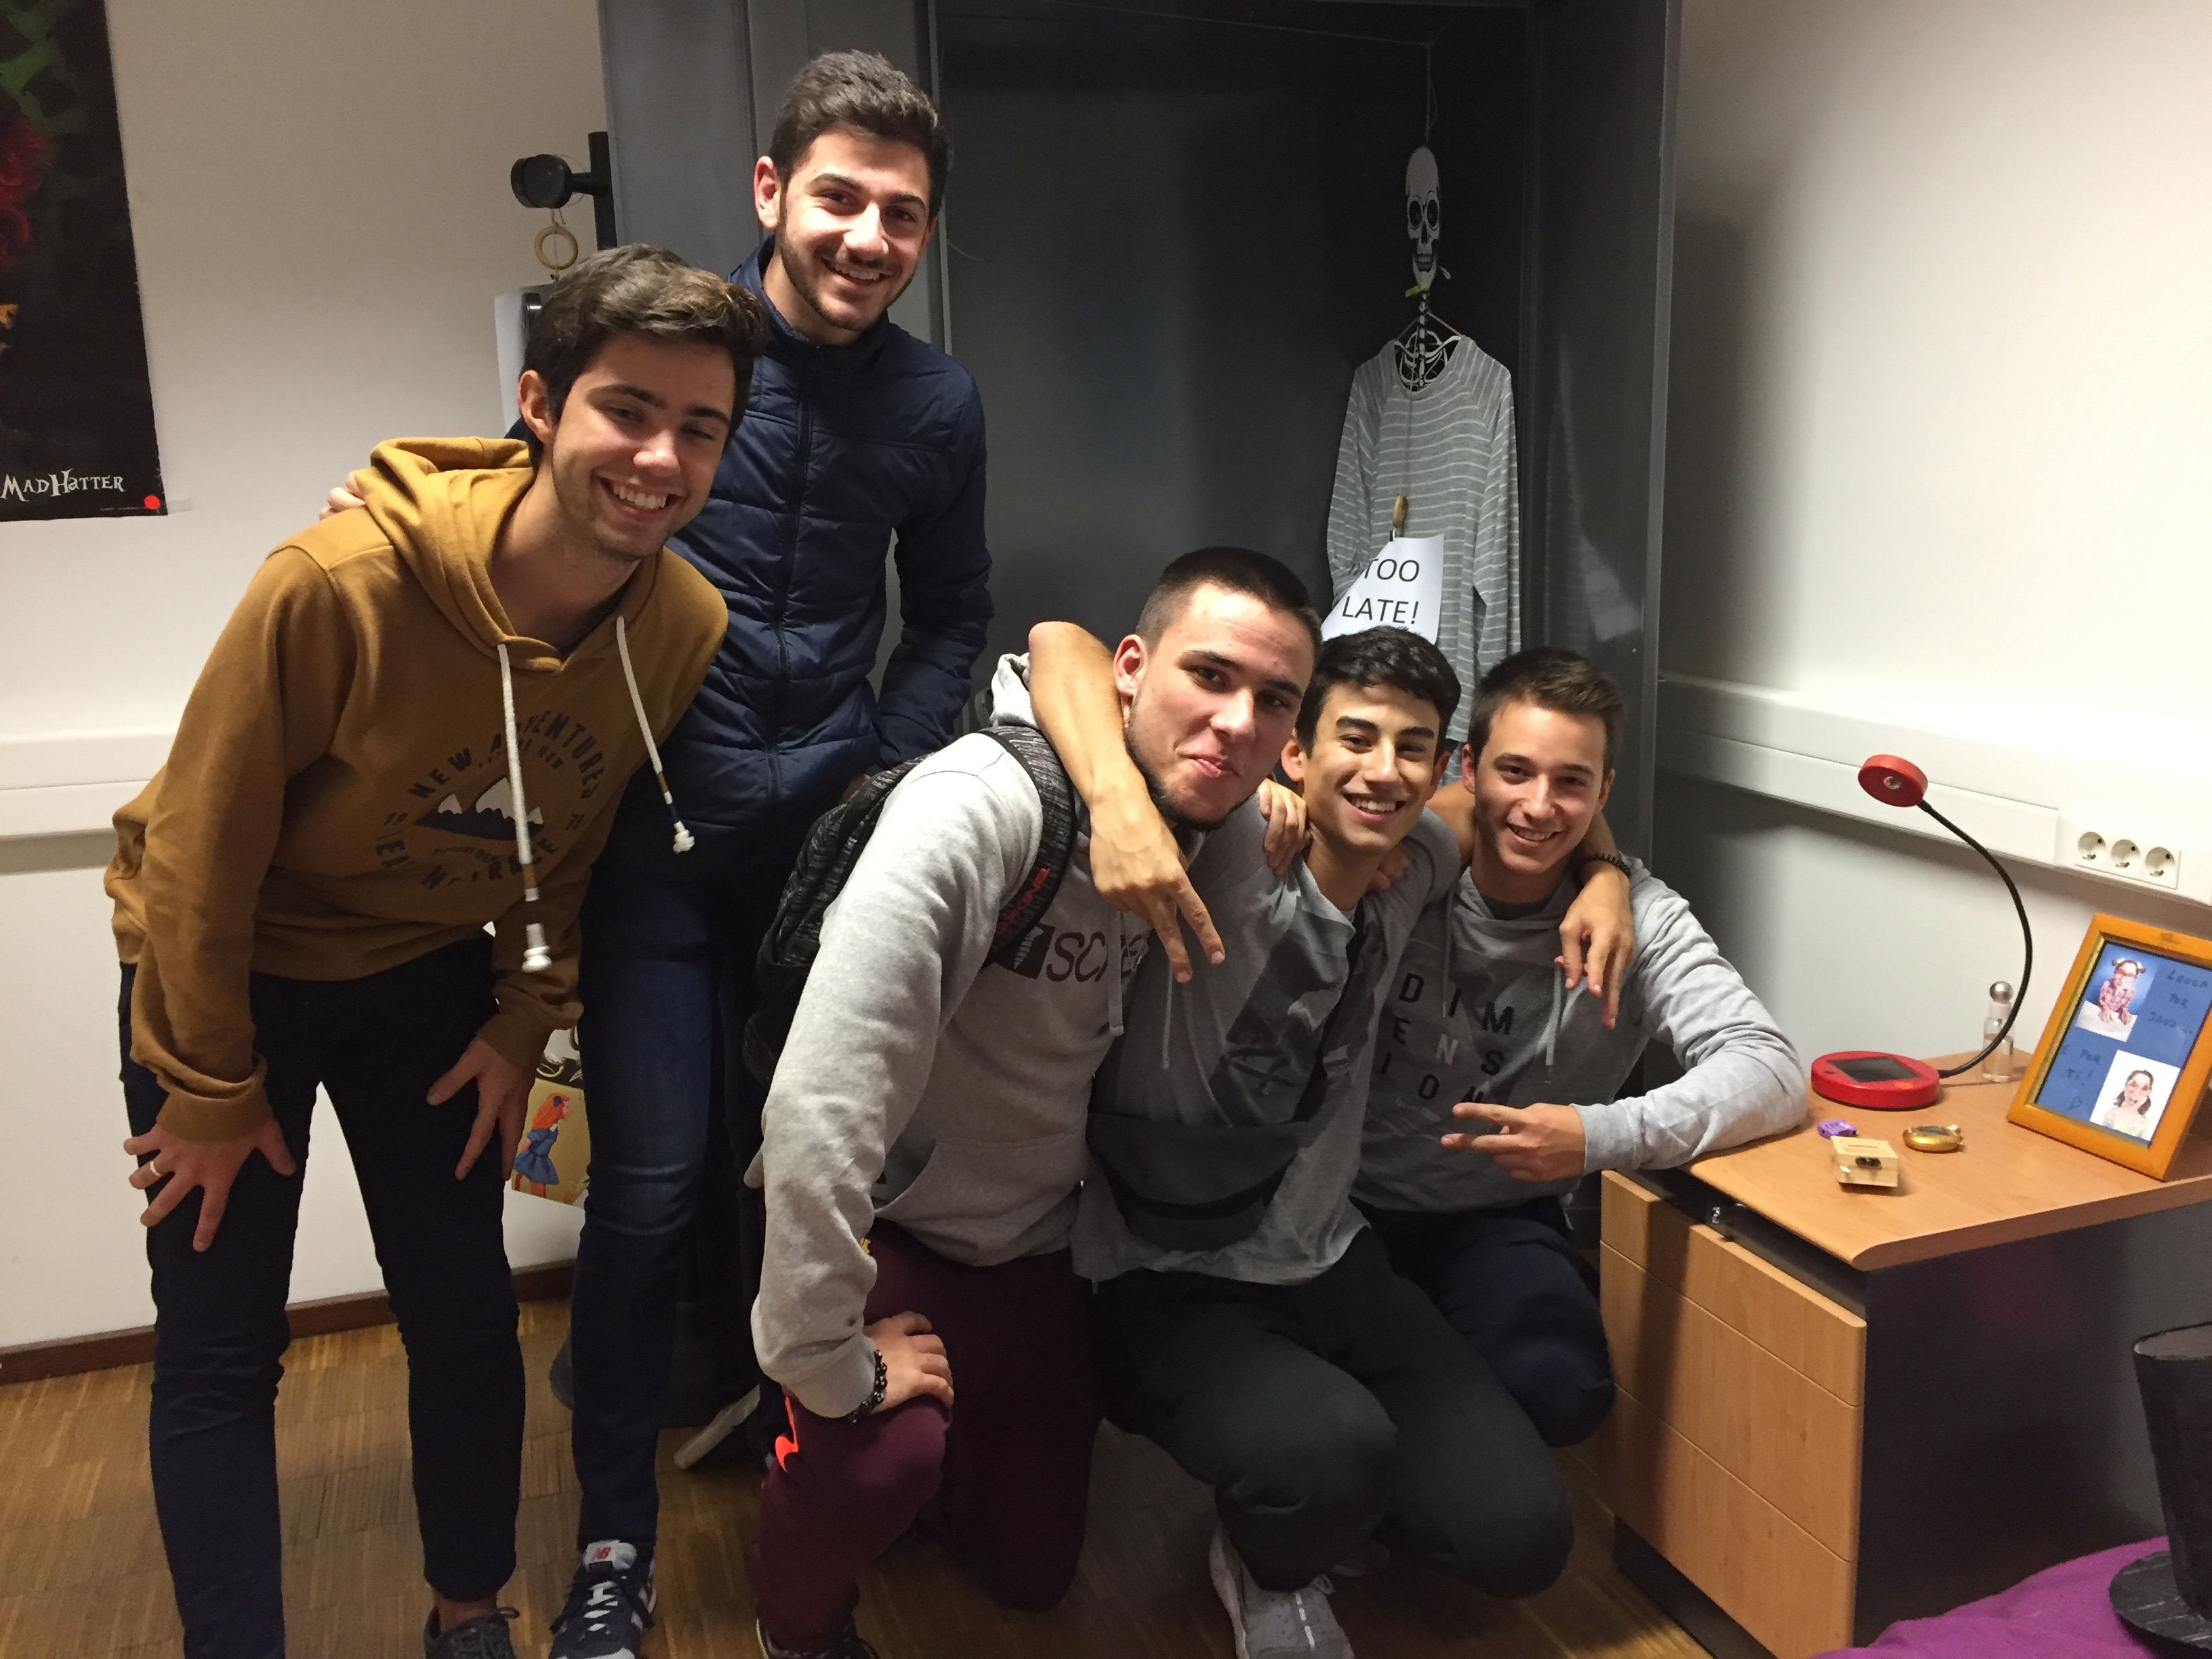
\includegraphics[width=.9\textwidth]{chaps/Images/IMG_3002(1).jpeg}
    \caption{Quase todos os alunos tiraram uma foto ao lado do esqueleto de Anita no armário.}
    \label{fig:quarto_anita_esqueleto}
\end{figure}

Em termos de cenário, a simplicidade também é a melhor política, pois tornará a experiência mais barata, e os organizadores não irão perder tempo procurando objetos específicos para comprar. No entanto, é fundamental ter objetos que caracterizem o espaço (como a cama e os pertences pessoais de Anita). Neste cenário particular de um quarto de meninas, adicionamos fotos de seu namorado, perfume e livros para jovens adultos. Um esforço para corresponder ao universo dos alunos atuais é altamente recomendado. Sabíamos, a partir de conversas com alunos, que a maioria tinha assistido "Vingadores: Endgame" da Marvel na época e adicionado várias referências ao filme no cenário. Por exemplo, na foto de Anita com o namorado, acrescentamos o texto “te amo 3000”, a frase que o Homem de Ferro diz para a filha. Essas referências foram mencionadas positivamente durante os debriefings e nos comentários dos questionários. Além disso, muitos alunos leram os livros de Harry Potter e também adicionamos referências a eles. No que diz respeito à dinâmica do jogo, um elemento comum do EG ao vivo é o game master (alguém que apresenta a atividade e orienta os participantes). Decidimos não ter um game master por três motivos. Em primeiro lugar, pensamos que os alunos prefeririam jogar o jogo sem um professor por perto, mesmo que remotamente. Em segundo lugar, havia limitações de tempo dos professores. Por fim, também é relatado que o papel do corpo docente na atividade pode ser confuso a princípio - por um lado, é necessário dar instruções claras e suficientes para que os alunos saibam o que fazer, minimizando a frustração \citep{hermanns_using_2017} e ajudar os alunos quando eles estão presos e não podem progredir \citep{borrego_room_2017}; por outro lado, dar muitas instruções pode reduzir a dificuldade do jogo a um ponto em que se torna uma fonte de tédio. Em ambientes educacionais, ambas as situações devem ser evitadas \citep{vahldick_dynamic_2017}, pois o nível de desafio representa um fator importante para a ludicidade de um jogo \citep{hong_playfulness-based_2009}.

Portanto, em vez de ter alguém dando instruções, optamos por:

\begin{itemize}
    \item Simplifique o fluxo do jogo, oferecendo aos alunos um desafio de cada vez. Em participantes regulares do EG
    \item Gaste tempo tentando entender qual desafio deve ser resolvido e como tudo é combinado. Aqui, e como o principal objetivo era fazer com que os alunos praticassem diferentes tipos de exercícios, foram propostos desafios um a um. Cada vez que um desafio era resolvido, os alunos teriam informações suficientes para identificar e resolver o próximo desafio. Forneça os materiais do curso na mesa de Anita, para os alunos podem estudar qualquer assunto, se necessário. Como dito anteriormente, em nosso piloto, as soluções dos exercícios estavam disponíveis e os alunos poderiam verificá-las se necessário. Em EscapulISTe? -LA, um livro de Álgebra Linear estava disponível.
\end{itemize}

Além disso, para não limitar o jogo a abrir e fechar armários, investimos em materiais como luz negra, pintura invisível e ímãs que são acessíveis e podem levar a experiências engraçadas. Como último conselho, faça o máximo de testes possível. Por exemplo, em EscapulISTe? -LP, nossos testadores descobrem que um dos códigos pode ser recuperado sem resolver o exercício até o final. Em EscapulISTe? -LA, os testadores descobriram que a mesma chave poderia abrir o armário e a gaveta da mesa de cabeceira.

\subsection{Conclusão e Próximos Passos}

Neste seção, a implementação de dois EEGs foi descrita. Avaliamos a experiência e concluímos que os alunos se engajam nesse tipo de atividade, têm consciência dos ganhos de aprendizagem e valorizam-na como uma experiência de aprendizagem frutífera. Esta atividade foi enquadrada no paradigma de aprendizagem ativa e, embora demorada para os professores, foi um complemento valioso para as aulas regulares. Como trabalho futuro, exploraremos como adaptar um enredo / cenário definido a um novo curso. Se a interface entre o designer e o especialista em conteúdo estiver bem definida, é um processo fácil personalizar os desafios para um curso diferente. Além disso, exploraremos a ideia de criar jogos de tabuleiro de fuga educacional.


\section{Mapeamento Sistemático de Autorregulação da Aprendizagem}

\section{Análise de dados no MOOC Técnico}

Neste relatório faz-se a análise de dados de três edições consecutivas dos cursos online “Controlo e Simulação de Drones” (droneX) e “Transformação Digital” (tdX), disponibilizados na Plataforma MOOC Técnico 1 . No primeiro caso, droneX, referimonos às edições de 2018, 2019 e 2020 e no segundo , tdX, considerámos as edições de 2017, 2018 e 2020. O nosso objetivo é analisar o comportamento de adesão dos 2
estudantes do Técnico Lisboa e de participantes externos inscritos nestes MOOC às atividades de avaliação, identificando padrões no seu desempenho, em particular com base no género, fazendo uma análise conhecida como Learning Analytics, Analytics e acrescentar alguns comentários individuais desses participantes enquanto avaliadores das atividades e conteúdos do droneX e do tdX. A análise com base no gênero é importante 3 no contexto da participação do MOOC Técnico no projeto
europeu FOSTWOM (2019). Este projeto tem como objetivo principal atuar na falta de equilíbrio de género nas áreas STEM, usando o potencial democrático dos MOOC.

Para a análise de dados usamos as pautas das avaliações para cada uma das edições
MOOC (em formato .csv) e fichas de perfil dos inscritos (em formato .csv), ambas
geradas pela plataforma e retiradas no final de cada edição. Incluímos ainda dados de
questionários iniciais e questionários finais. Estes últimos são respondidos via Google
Forms, mas acedidos diretamente na plataforma em cada uma das edições droneX e tdX. Como contextualização indicamos os objetivos gerais, o público alvo e a organização das atividades de avaliação, em cada um dos casos, droneX e tdX. Pontualmente, foram analisados os arquivos das pautas finais do Fénix  da UC  de “Controlo de Voo” para comparação de números de estudantes inscritos nesta UC com números totais de inscrições no MOOC droneX.

Para a análise,
escolhemos os seguintes para tratar os seguintes indicadores: taxa de Completion Rate
sucesso (Completion Rate) no MOOC em cada uma das edições sucessivas dos dois cursos online; distribuição de participantes por género em cada uma das edições; número de participantes inscritos com filiação IST; taxa de sucesso relativo por género, ou seja, participantes femininos/masculinos com sucesso entre participantes inscritos femininos/masculinos; comentários de satisfação dos participantes quanto às atividades avaliativas e quanto às expectativas iniciais sobre o MOOC (dados
qualitativos).

Na realização das análises mais estruturadas usámos RStudio, que é um software
livre de ambiente de desenvolvimento integrado para linguagem R. A linguagem R é uma linguagem de programação que permite gerar gráficos com base em cálculos estatísticos, permitindo-nos analisar dados agregados provenientes de ficheiros diferentes. É importante destacar que os números apresentados neste relatório provêm de ficheiros (.csv) diferentes, provenientes da plataforma MOOC Técnico, que foram posteriormente agregados para serem tratados no RStudio. Foram agregados em cada caso, droneX e tdX, três ficheiros tipo grade e três ficheiros tipo profile, descarregados a partir da plataforma em datas imediatamente posteriores ao final de cada edição. Numa primeira etapa, os dados agregados foram limpos, uma vez que
enrollees com registos no ficheiro grade que não existem participantes inscritos (enrollees)
estão no ficheiro profile, profile e vice-versa. A agregação feita no RStudio dos seis ficheiros de cada curso online foi feita com base nos indicadores “id”, “username”,
“email”,“ano”(by=c('id','username','email','ano')) através do comando join . Assim, o RStudio
gera relatórios finais com números totais por curso online e por ano, por género, por
Completion rates) rates global ou parcial, por exemplo, usando os dados taxas de sucesso (Completion primários que se comportam bem para os indicadores referidos. Os números gerados
pelo RStudio, e que apresentamos neste relatório, são números que se referem a
estes últimos dados primários.

\subsection{Contexto do MOOC Simulação e Controlo de Drones (droneX)}

O MOOC “Simulação e Controlo de Drones” (droneX) é aconselhado aos estudantes
inscritos na UC “Controlo de Voo” e usado durante os semestres de execução desta
UC numa estratégia de flipped-classroom
flipped-classroom. Em particular, o resultado das atividades de avaliações do MOOC contaram em cada uma das suas edições com uma
percentagem para a nota final da UC, que é uma disciplina do 3o ano do Mestrado Integrado de Engenharia Aeroespacial. Como se pode ler na página About o curso online droneX tem como objetivo analisar o funcionamento de drones multirotores e das partes que os constituem,
saber como desenvolver um simulador para analisar o seu comportamento e projetar soluções para o seu controlo automático.
As atividades de avaliação do MOOC droneX nas suas últimas três edições consistiram em um teste de avaliação de conhecimentos relativo a cada um dos quatro módulos, e um exame final, com questões de escolha múltipla e exercícios
vários, em que cada avaliação contou com 20\% para a nota final. Quando um participante atinge pelo menos 60\% de sucesso nas atividades avaliativas do curso, recebe um Honor Certificate correspondendo a um certificado de participação no curso com sucesso (sem classificação atribuída). É com base no número de certificados emitidos que se calcula a taxa de sucesso no MOOC.


\subsection{Análise dos dados de três edições}

Estiveram inscritos na edição do droneX de 2018 um total de 1258 participantes, entre os quais 424 inscreveram-se mediante autenticação Fénix com IST ID. Nesta edição, inscreveram-se 160 participantes do género feminino, dos quais 50 participantes tiveram sucesso (pelo menos 60\% de sucesso) nas atividades de avaliação do MOOC. Com relação ao género masculino, o total de participantes inscritos foi de 1088, 14 dos quais 312 participantes tiveram sucesso. O número total de participantes femininos e masculinos que terminaram com sucesso em 2018 foi de 362, o Completion rate que resulta numa taxa de sucesso (Completionrate) geral de 29\%.

Em 2019, estiveram inscritos no droneX um
total de 428 participantes, entre os quais 341
inscreveram-se com a autenticação Fénix. Deste número, 69 participantes eram do género feminino, tendo 28 participantes terminado com sucesso. Com relação ao género masculino, o total de participantes foi de 357, tendo 150 participantes terminado com sucesso. O total de participantes femininos e masculinos que tiveram sucesso foi de 178 de participantes femininos e masculinos que tiveram sucesso foi de 178, o que resulta numa Completion rate
taxa de sucesso (Completionrate) total 42\%.

Em 2020, estiveram inscritos 518 participantes,
entre os quais 458 inscreveram-se com a
autenticação Fénix. Nesta edição do droneX,
inscreveram-se 91 participantes do género
feminino das quais 53 foram as participantes
femininas que tiveram sucesso. Com relação ao
género masculino, o total de participantes foi de 420, dos quais 213 tiveram sucesso. O número de participantes femininos e masculinos que
terminaram com sucesso foi de 266, resultando
Completion rate numa taxa de sucesso (Completion rate) geral de 51\%, a mais elevada até ao momento.

\begin{figure}
    \centering
    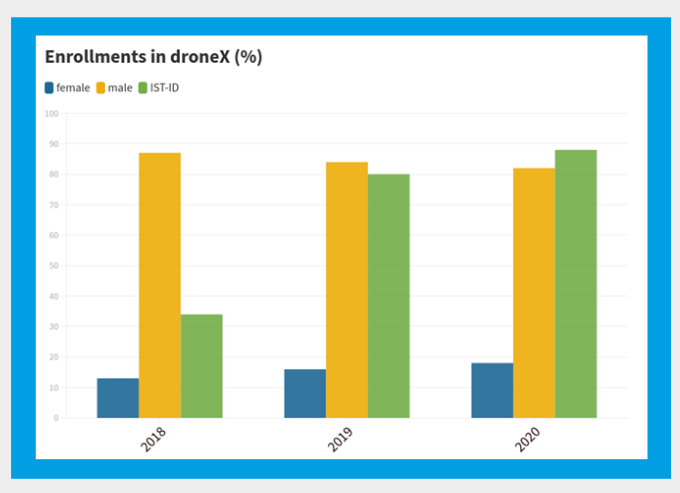
\includegraphics[width=.9\textwidth]{chaps/Images/taxa_insc_dronex.png}
    \caption{Taxas de inscrição nas várias edições do droneX}
    \label{fig:taxa_insc_dronex}
\end{figure}

Na Figura 1, podemos ver a distribuição
em cada ano da taxa de inscrição no
droneX por género (female, male) e a female, male percentagem de inscritos com filiação
IST (IST-ID), que neste caso pode indicar também estudantes inscritos na UC “Controlo de Voo” (ver ainda Fig. 5), ou alumni.

\begin{figure}
    \centering
    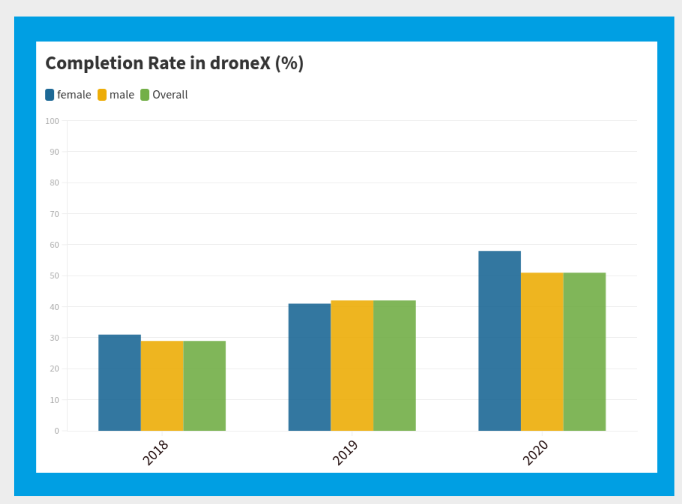
\includegraphics[width=.9\textwidth]{chaps/Images/taxa_sucesso_dronex.png}
    \caption{Taxas de sucesso nas várias edições do droneX.}
    \label{fig:taxa_sucesso_dronex}
\end{figure}

Na Figura 2, podemos ver as taxas de
sucesso (Completion rates) em cada Completion rates edição anual do droneX, percentagens
female, male género (female, female, por female, male male) e a overall percentagem total Overall A partir dos dados referidos
(Overall). acima e da visualização das duas
figuras, podemos concluir que a maioria dos inscritos no droneX são estudantes IST ou alumni do género masculino, e veremos na secção Flipped classroom com UC do Técnico  que só alguns deles são também estudantes inscritos na UC “Controlo
de Voo”.

As taxas de sucesso no droneX, exceto a total e a do género masculino na edição de 2018, situam-se acima dos 30\%. As taxas de sucesso femininas (relativas às inscrições femininas) em 2018 e 2020 ultrapassam as taxas globais.

\begin{figure}
    \centering
    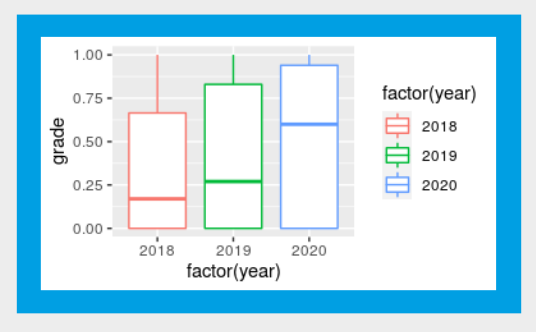
\includegraphics[width=.9\textwidth]{chaps/Images/boxplot_grade_dronex.png}
    \caption{Boxplot para a variável grade por fator year. Para cada caixa temos uma base que representa o primeiro quartil, um traço dentro da caixa que representa a mediana e o segundo quartil simultaneamente, e o topo da caixa que
representa o terceiro quartil.}
    \label{fig:boxplot_grade_dronex}
\end{figure}

No diagrama boxplot da Figura 3 podemos ver a relação entre as notas (numa escala de 0\% a 100\%) dos participantes no curso online droneX ao longo de três anos (2018, 2019 e 2020), com os dados agrupados de grade em relação ao fator year year. Verifica-se uma assimetria positiva para os dados de 2018 e 2019 e uma
assimetria negativa para os dados de 2020. É
importante notar que a mediana (segundo quartil) e o terceiro quartil das notas obtidas no MOOC tem vindo a aumentar ao longo destes três anos, estando em 2020 a
mediana próxima de 60\% e o terceiro quartil próximo dos 94\%. Recordamos que esta última edição decorreu durante um semestre académico marcado pela pandemia Covid-19, em que as aulas e a avaliação passaram para um regime remoto. O interesse e relevância de conteúdos online, em particular os MOOC, aumentaram substancialmente entre o público universitário. A caixa correspondente a 2020 é disso testemunho.

\begin{figure}
    \centering
    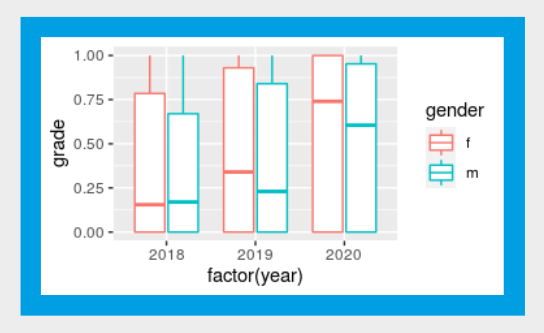
\includegraphics[width=.9\textwidth]{chaps/Images/boxplot_gender_drone.png}
    \caption{Boxplot para as variáveis grade e gender por fator year.}
    \label{fig:boxplot_gender_dronex}
\end{figure}

No diagrama boxplot da Figura 4, podemos ver a
relação entre as notas (numa escala de 0\% a
100\%) dos participantes no curso online droneX agrupados por grade e gender (f=feminino e m=masculino) em relação ao fator year (anos 2018, 2019 e 2020). Verifica-se que as assimetrias por género seguem o mesmo padrão dos dados globais, sendo positivas para os ambos os géneros em 2018 e 2019, e negativas para ambos os géneros em 2020. É importante notar que a mediana (segundo quartil) e o terceiro quartil das notas obtidas pelos participantes do droneX têm vindo a aumentar ao longo destes três anos.

Em geral, as medianas e os valores do terceiro quartil das notas de participantes femininas em 2019 e 2020 são mais elevadas do que as dos participantes masculinos. Por exemplo, em 2020 a mediana feminina encontra-se nos 74\%,
enquanto a mediana masculina está próxima de 61\%, e o terceiro quartil feminino próximo dos 100\%, enquanto o terceiro quartil masculino se encontra próximo dos 97\%. A edição de 2020 foi aquela em que houve mais participantes inscritos com sucesso nas atividades de avaliação, em particular houve muitas notas de participantes femininas próximas dos 100\%.

\subsection{Flipped classroom com
UC do Técnico Lisboa}

Para uma breve comparação entre os dados de inscrições e taxa de sucesso do droneX e da disciplina “Controlo de Voo” fornecem-se os
números abaixo. Dos participantes inscritos nas três edições referidas do MOOC droneX, um
número de 141 participantes em 2018, de 120 em 2019 e de 139 em 2020, eram também estudantes inscritos na UC “Controlo de Voo”.

De entre os 141 estudantes da UC “Controlo de Voo” de 2018, 23 estudantes eram do género feminino, dos quais 4 participantes terminaram com sucesso o droneX. Com relação ao género masculino, 119 estudantes participaram, sendo 7 os que finalizaram com sucesso.

Em 2019, o número total de estudantes inscritos na UC foi de 120. Destes, 23 estudantes eram do género feminino, e 20 destas participantes tiveram sucesso
no droneX. Com relação ao género masculino, 97
estudantes participaram, sendo 72 os que
obtiveram sucesso.

\begin{figure}
    \centering
    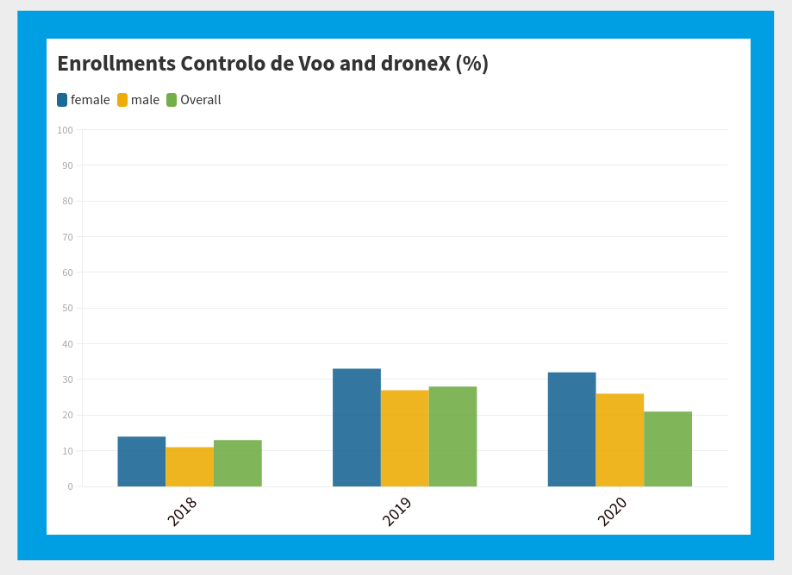
\includegraphics[width=.9\textwidth]{chaps/Images/enrollments_voo_drone.png}
    \caption{Percentagens de inscrição de estudantes da UC no droneX.}
    \label{fig:enrollment_voo_dronex}
\end{figure}

Em 2020, o número total de estudantes inscritos em “Controlo de Voo” foi de 139, dos quais 29 estudantes eram do género feminino. Destas, 27 estudantes ao participarem no droneX, obtiveram sucesso contribuindo para a
mediana próxima dos 75\% referida acima (ver
Fig. 4). Com relação aos inscritos masculinos na UC, 110 participaram no droneX, com 82 entre eles que obtiveram sucesso nas atividades de avaliação.

\subsection{Conclusão sobre a experiência global do MOOC droneX}

Podemos assim concluir que os participantes inscritos nas várias edições do droneX são estudantes IST ou 19 alumni de género masculino, mas só alguns deles são também estudantes inscritos na UC “Controlo de Voo”
(ver Fig. 5).

Relativamente à prestação feminina das várias edições do droneX, queremos sublinhar que embora exista uma percentagem baixa de alunas inscritas na UC de "Controlo de Voo” (entre 16\% e 21\%), e também de participantes femininas no MOOC (ver Fig. 1), estas
últimas alcançaram boas taxas de sucesso no droneX (ver Fig. 4). Recordamos que um dos objetivos principais do projeto europeu FOSTWOM é chamar a atenção para a falta de equilíbrio de género em muitas áreas STEM e
usar a acessibilidade dos MOOC para aumentar a
participação feminina nas áreas de Engenharia.

De modo geral, os participantes demonstraram
estar satisfeitos com as atividades de avaliação e os conhecimentos adquiridos.

Deste modo, quando se desenha e produz um MOOC a pensar em usá-lo como complemento, ou mesmo em aplicá-lo em flipped-classroom a uma UC específica do Técnico Lisboa, está a servir-se uma comunidade académica da escola mais alargada, como estudantes de outras UC e/ou alumni.

\subsection{ANÁLISE DO CURSO ONLINE TRANSFORMAÇÃO DIGITAL}

\subsection{Contexto do MOOC Transformação Digital}

O MOOC “Transformação Digital” (tdX), como se pode ler na descrição da About é aconselhado a todos os profissionais, alunos finalistas
sua página About, (prestes a entrar no mercado de trabalho) e ainda a potenciais empreendedores que tenham interesse em perceber o papel das novas tecnologias nas
organizações, tanto públicas como privadas Os participantes neste curso deverão ter interesse pelas novas tecnologias assim como vontade de transformar as organizações onde trabalham atualmente e/ou criar novos negócios.

Dentro do contexto MOOC Técnico, este MOOC é um curso online transversal para um público alargado, não obrigatoriamente académico, que tem como propósitos tirar partido das novas tecnologias para transformar as organizações, tendo como objetivo final aumentar as vendas, reduzir custos, ou criar novos negócios.

As atividades de avaliação do MOOC tdX nas suas últimas três edições consistiram em 4 exercícios de Peer Review Review. Estes exercícios são enunciados no final de cada tópico. Os participantes devem responder individualmente, sendo as respostas submetidas posteriormente avaliadas pelos seus pares, pequeno grupo de constituição aleatória de outros participantes inscritos. Finalmente, há uma revisão e confirmação da classificação mediana do grupo feitas pelo tutor.
Quando um participante atinge pelo menos 60\% de sucesso nas atividades avaliativas de Peer Review Review, recebe um Honor Certificate
Certificate, certificado de participação com sucesso (sem classificação atribuída). Recordamos que é com base no número de certificados emitidos que se calcula a taxa de sucesso no MOOC.

\subsection{Análise dos dados de três edições}

Em 2017, estiveram inscritos no tdX um total
de 1111 participantes, em que 78\% dos
participantes eram externos ao Técnico Lisboa.
Do total de participantes, 317 corresponderam a inscrições de género feminino, sendo 61 as
participantes femininas que obtiveram sucesso
(pelo menos 60\% de sucesso) nas atividades
de avaliação. Com relação ao género masculino,
21 o total de inscritos masculinos foi de 785, dos quais 162 inscritos obtiveram sucesso. O
número total de participantes que obtiveram
sucesso foi de 223, o que resulta numa taxa de
Completion Rate) geral de 20\%.

Estiveram inscritos na edição do tdX de 2018 um total de 1046 participantes, em que 73\% dos
participantes eram externos ao Técnico Lisboa.
Entre os inscritos, 336 participantes eram do
género feminino, sendo 50 as participantes que
obtiveram sucesso. O total de participantes de
género masculino foi de 707, com 137 destes
participantes a obterem sucesso nas atividades
de avaliação. O número de participantes
femininos e masculinos que obtiveram sucesso
foi de 187, o que resulta numa taxa de sucesso
Completion Rate (Completion Rate) geral de 18\%.

Em 2020, estiveram inscritos no total 1405
participantes, sendo que de novo 78\% dos
participantes eram externos ao Técnico Lisboa.
Nesta edição, 544 participantes eram do género
feminino, sendo 173 as participantes que
obtiveram sucesso. O total de participantes de
género masculino foi de 857, com 278 entre eles a obterem sucesso nas atividades de avaliação. O número de participantes femininos e masculinos que obtiveram sucesso foi de 451, o que resulta Completion Rate numa taxa de sucesso (Completion Rate) geral de 32\% que se aproxima da taxa de sucesso média de um curso MOOC Técnico.

\begin{figure}
    \centering
    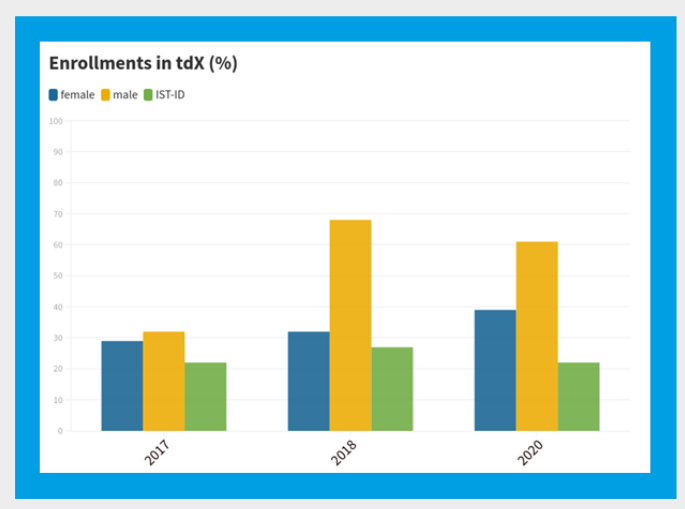
\includegraphics[width=.9\textwidth]{chaps/Images/enrollments_tdx.png}
    \caption{Taxas de inscrição nas várias edições do tdX.}
    \label{fig:enrollment_tdx}
\end{figure}

Na Figura 6, podemos ver a distribuição em cada ano da taxa de female, inscrição no tdX por género (female, male male) e a percentagem de inscritos com filiação IST (IST-ID), que neste caso é bastante inferior à percentagem
dos restantes inscritos, e bastante inferior aos valores das percentagens de inscrições com filiação IST no curso online droneX (ver Fig. 1 para os anos 2019 e 2020).

\begin{figure}
    \centering
    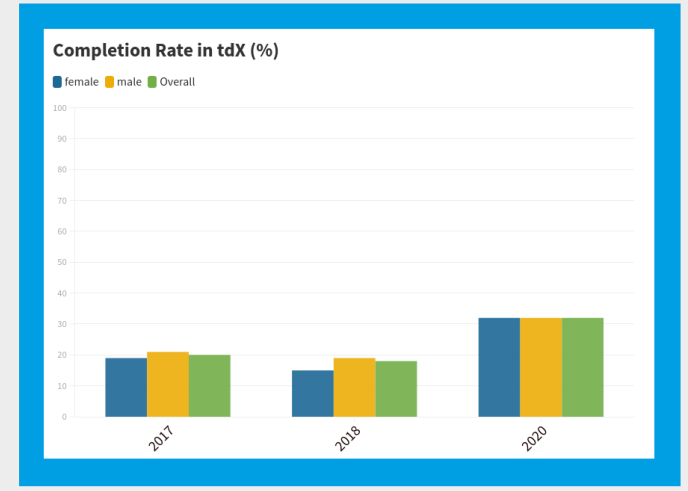
\includegraphics[width=.9\textwidth]{chaps/Images/completion_rate_tdx.png}
    \caption{Taxas de sucesso nas várias edições do tdX.}
    \label{fig:rate_tdx}
\end{figure}

Na Figura 7, podemos ver as taxas de sucesso (Completion rates) em cada Completion rates edição anual do tdX,as percentagens female, male género (female, female, por female, male male) e a overall percentagem Overall A partir dos dados total (Overall). referidos acima e da visualização das duas últimas figuras, podemos concluir que a maioria dos inscritos
no tdX são participantes externos ao IST de género masculino. As taxas de sucesso no tdX situam-se entre os 18\% e os 32\%, sendo que na última edição de 2020, todas as taxas de Overall female, male sucesso (Overall,
male) são iguais a este valor máximo de 32\%.

\begin{figure}
    \centering
    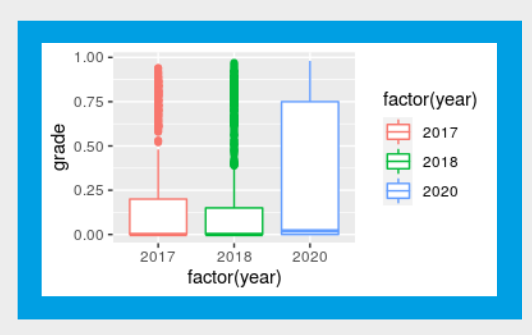
\includegraphics[width=.9\textwidth]{chaps/Images/boxplot_grade_tdx.png}
    \caption{Boxplot para a variável grade por fator year. Para cada caixa temos uma base que representa o primeiro quartil, um traço dentro da caixa que representa a mediana e o segundo quartil simultaneamente, e o topo da caixa que
representa o terceiro quartil. Os pontos isolados correspondentes às caixas vermelha e verde são outliers.}
    \label{fig:boxplot_grade_tdx}
\end{figure}

No diagrama boxplot da Figura 8, onde se pode ter uma leitura mais fina das taxas de sucesso relativas às notas obtidas pelos participantes, pode ver-se a existência de
muitos outliers outliers, principalmente nas duas primeiras edições 2017 e 2018 do tdX. Torna-se mesmo difícil de ler a mediana para esses dois anos, assim como a mediana
de 2020 que também está próxima de 2\% (numa escala de 0\% a 100\%) conferindo uma acentuada assimetria positiva nessas duas caixas. As caudas de distribuição, ou seja, as distâncias entre o terceiro quartil e o último
outlier, das notas para 2017 e 2018 também são grandes.

É importante recordar que a taxa de sucesso (Completion embora as referidas medianas se situem em valores muito baixos. Pode acontecer que o Peer Review resulte mais penalizante do que o tipo de avaliação usado no droneX. Na caixa respeitante à edição 2020 já não se visualizam outliers, outliers embora a dispersão das notas seja grande e o terceiro quartil fique nos 75\%. Recordamos que a última edição decorreu durante um período marcado pela pandemia Covid-19, em que o interesse e relevância de conteúdos online, em particular os MOOC, aumentaram substancialmente entre o público em geral. Os números de retenção desta edição 2020 do tdX
testemunham esta tendência.

\begin{figure}
    \centering
    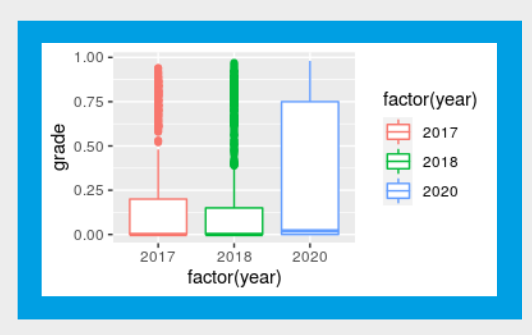
\includegraphics[width=.9\textwidth]{chaps/Images/boxplot_grade_tdx.png}
    \caption{Boxplot para as variáveis grade e gender poryear fator year.}
    \label{fig:boxplot_gender_tdx}
\end{figure}

No diagrama boxplot da Figura 9, verifica-se uma assimetria positiva muito acentuada dos dados de grade e gender (f=feminino e m= masculino) em relação ao fator year (anos 2017, 2018 e 2020) do curso online de tdX, principalmente nas caixas correspondentes às notas de participantes femininas. É possível ver com base na distribuição por género
das notas (numa escala de 0\% a 100\%) dos
participantes femininos e masculinos inscritos no tdX ao longo desses três anos, que as medianas se situam muito próximo dos 0\% em ambos os casos, sendo que na edição 2020 a mediana das notas dos participantes masculinos é próxima de 3\%.

A edição de 2020 foi aquela em que houve mais participantes inscritos que terminaram com sucesso as atividades de avaliação, em que o terceiro quartil das notas para o género masculino é de cerca de 75\%, igual ao valor do terceiro quartil global desta edição (ver Fig. 8).

\subsection{Conclusão sobre a experiência global do MOOC tdX}

Finalmente, concluímos que a maioria dos inscritos nas várias edições do tdX são participantes externos ao IST de género masculino.

Relativamente à prestação feminina nas várias edições do tdX , notamos que existe uma percentagem ligeiramente mais baixa de participantes femininas com sucesso no
MOOC (ver Fig. 7), excepto em 2020, em que a taxa de sucesso é igual para ambos os géneros. Eventualmente para esta tipologia de MOOC extracurricular faz mais sentido fazer outro tipo de análise com base noutros indicadores.

De modo geral, o público alargado, não obrigatoriamente académico, inscrito nas várias edições do curso online demonstrou estar satisfeito com as atividades de avaliação Peer Review), Review bem como com os conhecimentos adquiridos durante o curso.

Fica aqui a recomendação para se estudarem estratégias de captação e retenção de um público externo à escola, aplicando metodologias ativas que ajudem a aumentar as
taxas de sucesso nesta tipologia de MOOC transversal, com a ressalva que estas estratégias dependem muito do tópico
escolhido para o curso online, obviamente.

\subsection{Conclusão final das análises dos dados}

Terminada a análise separada sobre os dois MOOC com características distintas: o
curso “Simulação e Controlo de Drones”, droneX, dirigido principalmente a um
público de perfil “estudante IST”, e o curso “Transformação Digital”, tdX, dirigido a
um público alargado, conclui-se que a adesão às atividades de avaliação, enquanto
indicador do comportamento de adesão dos participantes a cada um dos tipos de
MOOC é também bastante distinta. Enquanto o droneX, aconselhado aos estudantes inscritos numa UC do Técnico Lisboa e usado para apoiar uma estratégia de flipped-classroom
flipped-classroom, consegue ter uma taxa média de sucesso na ordem dos 41\%, o curso “Transformação Digital”, dirigido a um público menos académico, eventualmente profissionais e potenciais empreendedores, tem uma taxa
média de sucesso de 23\%.

De referir que enquanto o número de inscritos no tdX foi sempre superior a mil inscritos, com uma maioria de inscritos externos ao IST, no droneX só na primeira edição de 2018 o número de inscritos foi superior a mil
participantes. 

Gostaríamos de acrescentar que a divulgação das várias edições do tdX beneficiaram de alguns apoios externos, enquanto no caso do droneX a divulgação foi mais interna ao IST, exceto na edição de 2018.

O público de ambos os MOOCs é predominantemente masculino (ver Fig. 1 e 6), com uma forte assimetria no caso do
droneX. Os inscritos no droneX, sendo alguns deles estudantes inscritos na UC “Controlo de Voo” (ver Fig. 5), são maioritariamente do género masculino. No entanto, as taxas de sucesso relativas (Fig. 2) e as notas obtidas (Fig. 4) pelas participantes femininas nas edições do droneX são em média superiores quando comparadas com as dos seus colegas masculinos. No caso do tdX, embora não sendo uma tendência muito acentuada, o comportamento global é o inverso (ver Fig. 7 e 9).

De modo geral, os participantes inquiridos no final de cada edição demonstraram estar satisfeitos com as atividades de avaliação e os conhecimentos adquiridos em ambos os casos, droneX e tdX (secções 2.3 e 3.3). Recordamos ainda que as últimas edições de ambos os cursos que ocorreram respetivamente, em abril e maio de 2020, durante um
Completion Rates período marcado pela pandemia Covid-19, não só tiveram taxas de sucesso (Completion Rates) mais elevadas (Fig. 2 e
7), como em geral as notas obtidas pelos participantes que terminaram com sucesso foram mais altas (Fig. 3 e 8). A apetência por este tipo de conteúdos validados, com boa qualidade gráfica, possibilitando uma formação gratuita e de fácil acesso deverá ainda aumentar nos próximos tempos.

Finalmente, gostaríamos de comentar com base nos resultados da nossa análise que um curso MOOC Técnico desenhado para um público com perfil “estudante IST de uma dada UC”, como o droneX, consegue captar e servir ainda uma comunidade mais alargada, como estudantes de outras UC, estudantes internacionais e/ou alumni que procuram aprofundar, rever ou alargar os seus conhecimentos sobre o tópico. Enquanto isso, um curso transversal,
como o tdX, para além do público externo ao IST, não obrigatoriamente académico, consegue também oferecer gratuitamente à comunidade da escola conteúdos extracurriculares de qualidade.

\section{O Projeto IgualdadeStem}

\subsection{Dados analisados}

\subsection{Evento Jornada das Mulheres}

\subsection{Artigos publicados}

\subsection{Trabalhos apresentados}





